\begin{center}
\indent
\textit{Gruppi, anelli, campi. In particolare, anello degli interi modulo $m$ intero, anello dei polinomi.}
\end{center}

\section{Strutture algebriche con un'operazione}

Una struttura algebrica \`e una coppia $(A, \cdot)$ dove A \`e un'insieme e $\cdot$ (``per'') \`e un'operazione $\cdot : A \times A \to A$. Ad esempio $(\naturals, +)$ \`e una struttura algebrica.

Le operazioni sono funzioni definite su prodotti cartesiani a valori in un insieme. Un'operazione binaria \`e definita sul prodotto cartesiano fra due insiemi.

Riprendendo la composizione, dati tre insiemi $A, B, C$, $B^A$ \`e l'insieme delle funzioni da $A$ in $B$, $C^B$ \`e l'insieme delle funzioni da $B$ in $C$. La composizione $\circ$ \`e un'operazione definita sul prodotto cartesiano degli insiemi $B^A \times C^B$ in $C^A$ ($\circ : B^A \times C^B \to C^A$).

Posso rappresentare un'operazione come funzione $(\circ \left( f, g \right))$ o inserendo l'operatore fra i due operandi $ (g \circ f) $.
\begin{exmp}
\begin{align*}
f: \reals \times \reals \to \reals  & \, &
f(x,y) = \sqrt{2} \cdot x + y \\
g: \reals \to \reals \times \reals  & \, &
g(z) = (0,z) \\
g \circ f : \reals \times \reals \to \reals \times \reals & \, & 
(x,y) \xrightarrow{f} \sqrt{2} \cdot x + y = z \xrightarrow{g} \left( 0, \sqrt{2}x + y \right) \\
f \circ g : \reals \to \reals & \, &
z \xrightarrow{g} (0,z) \xrightarrow{f} \sqrt{2} \cdot 0 + z = z
\end{align*}
\end{exmp}

Una struttura algebrica \`e un'insieme su cui \`e definita un'operazione che prende due elementi di quell'insieme e gliene associa un terzo.

Le strutture vengono classificate in base alle loro propriet\`a:
\begin{description}
    \item[Propriet\`a associativa\label{itm:strutture_associativa}] $\forall a, b, c \in A : a \cdot (b \cdot c) = (a \cdot b) \cdot c$
    \item[Elemento neutro\label{itm:strutture_neutro}] Esistenza di un'elemento neutro, o elemento identit\`a. $1 \in A : \forall a \in A $, $a \cdot 1 = a = 1 \cdot a$
    \item[Propriet\`a commutativa\label{itm:strutture_commutativa}] $ \forall a, b \in A $, $a \cdot b = b \cdot a $. In una struttura algebrica commutativa in genere l'identit\`a si indica con 0.
    \item[Inverso\label{itm:strutture_inverso}] Esistenza dell'inverso. $ \forall a \in A \exists b \in A $ t.c. $a \cdot b = 1 = b \cdot a $.
\end{description}

\subsection{Classificazione delle strutture algebriche con una operazione}

Per essere studiabile, una struttura algebrica deve essere quantomeno associativa.

\begin{description}
    \item[Semigruppo] struttura algebrica associativa.
    \item[Monoide] struttura algebrica associativa con elemento identit\`a.
    \item[Gruppo] struttura algebrica associativa con elemento identit\`a e con inverso (ossia, monoide con inverso).
    \item[Gruppo abeliano] struttura algebrica che presenta tutte e quattro le propriet\`a: associativa, elemento neutro, commutativa, inverso.
\end{description}

La struttura algebrica $\left( \naturals, + \right)$ \`e un monoide commutativo. Anche $\left( \naturals, \cdot \right)$ \`e un monoide commutativo. $\left( \integers, + \right)$ \`e un gruppo perch\`e esiste l'inverso. $\left( \integers, \cdot \right)$ invece \`e un monoide, perch\'e non ha l'inverso per ogni elemento.

\subsection{Gruppo simmetrico\label{subsec:gruppo_simmetrico}}

\begin{defn}[Gruppo simmetrico]
Il prototipo di tutti i gruppi \`e il gruppo simmetrico su $n$ elementi, il cui insieme \`e indicato con $S_n$. Prendiamo un insieme $E = \left\{ e_1, \dots, e_n \right\}$.
\[
S_n = \left\{ f : E \to E \text{ t.c. $f$ \`e biunivoca} \right\}
\]
Quindi $S_n$ \`e l'insieme di tutte le permutazioni degli elementi di $E$. Il gruppo simmetrico \`e definito sull'insieme $S_n$ e l'operazione \`e la composizione: $\left( S_n, \circ \right)$. Verifica tutte le propriet\`a dei gruppi:
\begin{enumerate}
    \item $f \circ \left( g \circ h \right) = \left( f \circ g \right) \circ h$, ossia \`e associativo.
    \item L'unit\`a \`e la funzione identica (o identit\`a) $i_E : E \to E$ tale che $\forall e \in E $, $i_E(e) = e$
    \[
    f \circ i_E = f = i_E \circ f
    \]
    \item Una funzione biunivoca $f$ ha una funzione inversa $g$.
    \[
    g : E \to E \text{ t.c. } g \left( f(e) \right) = e
    \]
\end{enumerate}
\end{defn}

Una funzione $f : E \to E $ iniettiva su un insieme finito $E$ \`e necessariamente suriettiva e quindi biunivoca. Un insieme \`e finito se non pu\`o essere messo in corrispondenza biunivoca con un suo sottoinsieme proprio.

% \subsection{Punto di vista dell'occupazione}

% $f : \left \{ 1, \dots, 6 \right \} \to \left \{ 1, \dots, 6 \right \}$. Penso il dominio come degli oggetti. Il codominio come dei ``cassetti''. La funzione \`e un modo di mettere gli oggetti del dominio nei ``cassetti''.

% \begin{tabular}{cccccc}
% 1 & 2 & 3 & 4 & 5 & 6 \\
% 2 & 3 & 5  &1 & 6 & 4
% \end{tabular}
% \`E un'occupazione.

% \begin{tabular}{cccccc}
% 1 & 2 & 3 & 4 & 5 & 6 \\
% 6 & 6 & 3 & 5 & 5 & 5
% \end{tabular}
% Non \`e un'occupazione.


\section{Monoidi}

Un monoide $(M, \cdot)$ \`e una struttura algebrica con un'operazione $\cdot : M \times M \to M$ tale che:
\begin{description}
    \item[1M] L'operazione $\cdot$ \`e associativa;
    \item[2M] $\exists 1_M $ t.c. $ \forall a \in M$, $ 1_M \cdot a = a = a \cdot 1_M$, ossia esiste l'elemento identit\`a. 
\end{description}

Un sottomonoide $(S, \cdot)$ con $S \subseteq M$ \`e un monoide in cui esiste l'operazione $\cdot : S \times S \to S$, ossia $S$ \`e chiuso rispetto all'operazione $\cdot$, cio\`e $\forall s, s' \in S $, $s \cdot s' \in S$ e $1_M \in S$.

Ad esempio, considerando $(\naturals, +)$, il monoide $(P, +)$ con $P = \{ m \in \naturals : \exists k $ t.c. $m = 2k \}$ \`e un suo sottomonoide, perch\`e la somma di due pari \`e pari e lo 0 appartiene ai pari. I dispari con il + non sono un sottomonoide.

$k \naturals = \{ m \in \naturals : \exists t \in \naturals $ t.c. $ m = k t\}$ \`e la ``versione generale'' dell'insieme dei numeri pari.

Considerando $(\naturals, \cdot)$ e l'elemento neutro 1, i pari non sono un sottomonoide perch\'e non hanno l'elemento neutro, ma i dispari s\`i.

\subsection{Morfismi di monoidi}

\begin{defn}[Morfismo di monoidi]
Dati i monoidi $(M, \cdot)$ e $(A, \ast)$, un morfismo di monoidi \`e un'applicazione $f : M \to A$ che conserva le strutture, ossia tale che $\forall x,y \in M $ ho che:
\[
f(x \cdot y) = f(x) \ast f(y)
\]
Inoltre, $f(1_M) = 1_A$.
\end{defn}

\subsection{Teorema di omomorfismo per i monoidi\label{omomorfismo_monoidi}}

\begin{prop}
Sia $f : (M, \cdot) \to (A, \ast)$ un morfismo di monoidi, $f$ definisce una relazione di equivalenza $\varepsilon_f$ tale che $\ker f = M / \varepsilon_f \cong Im_f$, ossia il quoziente \`e isomorfo all'immagine. Inoltre il quoziente ha una struttura di monoide:
\[
(M / \varepsilon_f , \cdot) \cong (Im_f, \ast)
\]
con $(Im_f, \ast)$ sottomonoide di $(A, \ast)$.
\end{prop}
\begin{proof}
Ogni morfismo di monoidi $f : (M, \cdot) \to (A, \ast)$ individua un sottomonoide di $(A, \ast)$, che \`e $(Im_f, \ast)$. 

Essendo $f$ un morfismo di monoidi, $\forall f(x), f(y) \in Im_f$, $f(x) \ast f(y) = f(x \cdot y) \in Im_f$, quindi $Im_f $ \`e chiuso rispetto a $\ast$. Devo poi verificare che $1_A \in Im_f \Leftarrow f(1_M) = 1_A$.

Anche $(\ker f, \cdot)$ \`e un monoide. Dobbiamo dimostrare l'esistenza dell'isomorfismo con $Im_f$.

$\ker f$ \`e l'insieme delle classi di equivalenza $[x] = \{ y \in M : x \ \varepsilon_f \ y \iff f(x) = f(y) \} \in \ker f$.

Definiamo l'operazione di prodotto fra classi come la classe del prodotto di due rappresentanti $[x] \cdot [z] = [x \cdot z]$ qualsiasi rappresentante scelgo della classe. Bisogna verificare che questa definizione sia indipendente dai rappresentanti! Lo faremo nella sezione \ref{congruenze}, in particolare nella dimostrazione \ref{congruenza_monoidi}. % \`E verificato se $\varepsilon_f$ \`e una congruenza.

L'operazione fra classi \`e associativa, perch\'e \`e associativa l'operazione fra rappresentanti. Inoltre ho l'unit\`a $[1_M]$ in $\ker f$.

L'isomorfismo fra $(Im_f, \ast)$ e $(\ker f, \cdot)$ segue naturalmente dal fatto che $\ker f $ e $Im_f$ sono in biezione. Inoltre, essendo entrambi dei monoidi, la funzione $f$ \`e un isomorfismo di monoidi.
\end{proof}

\subsection{Potenze (iterazioni sui monoidi)}

\begin{defn}[Potenze]
A partire dal monoide $(M, \cdot)$ possiamo definire le iterazioni dell'operazione $\cdot$, ossia le potenze.

Sia $ a \in M$, si definisce:
\begin{enumerate}
    \item $a^0 = 1_M$
    \item $a^{n+1} = a \cdot a^{n}$
\end{enumerate}
\end{defn}
\begin{prop}[Commutativit\`a della potenza]
$\forall n \in \naturals$, $a \cdot a^n = a^n \cdot a$, ossia la potenza \`e commutativa.
\end{prop}
\begin{proof}
Si dimostra per induzione. Si vede subito che con $n = 0$, per definizione $a \cdot a^0 = a = a^0 \cdot a$.

Per definizione di potenza $a \cdot a^{n+1} = a \cdot a \cdot a^{n} $, per ipotesi induttiva $ a \cdot a^n \cdot a $ che di nuovo per definizione di potenza \`e $ a^{n+1} \cdot a$.
\end{proof}
\begin{prop}
Valgono tutte le propriet\`a tipiche delle potenze:
\[
a^{m + n} = a^m \cdot a^n
\]
\end{prop}
\begin{proof}
Si dimostra anche questo per induzione su $n$. Con $n = 0$, $a^{m+0} = a^m = a^m \cdot 1_M = a^m \cdot a^0$.

Passo induttivo: $a^{m + n + 1} = a \cdot a^{m + n}$ per definizione di potenze. Applicando l'ipotesi induttiva, $a \cdot a^{m + n} = a \cdot a^m \cdot a^n$. Per commutativit\`a $a \cdot a^m \cdot a^n = a^m \cdot a \cdot a^n = a^m \cdot a^{n+1}$.
\end{proof}

\begin{theorem}
Dato un monoide $(M, \cdot)$ ed un elemento $a \in M$, esiste un solo morfismo di monoidi $f : (\naturals, +) \to (M, \cdot)$ tale che $f(1) = a$, ed \`e $f(n) = a^n$.
\end{theorem}
\begin{proof}
$f$ \`e un morfismo di monoidi, quindi deve verificare che $f(m+n) = f(m) \cdot f(n)$ e che $f(0) = 1_M$. 

Per le propriet\`a delle potenze dimostrate precedentemente, $f(m+ n) = a^{m+n} = a^m \cdot a^n = f(m) \cdot f(n)$, e $f(0) = a^0 = 1_M$ per la definizione delle potenze. 

Inoltre verifica la condizione $f(1) = a$, infatti $f(1) = a^1 = a \cdot a^0 = a \cdot 1_M = a$.

Dobbiamo dimostrare l'unicit\`a di $f$. Sia $g : (\naturals, +) \to (M, \cdot )$ un morfismo tale che $g(1) = a$, dimostriamo che $\forall n \in \naturals $, $ g(n) = f(n) = a^n$.

Dimostriamolo per induzione su $n$. Per definizione di morfismo di monoidi, $g(0) = 1_M = f(0) = a^0$.

Supponiamo che $g(n) = f(n)$, per definizione di morfismo di monoidi $g(n+1) = g(1) \cdot g(n) = a \cdot g(n) = a \cdot f(n) = a \cdot a^n = a^{n+1}$.
\end{proof}

\begin{exmp}
Sia $\Gamma$ un insieme, la struttura algebrica $\left( \mathbb{P}(\Gamma), \cup \right)$ \`e in particolare un monoide. L'unione \`e associativa ($(A \cup B) \cup C = A \cup (B \cup C)$), ed esiste l'elemento neutro $\emptyset$.

Anche $\left( \mathbb{P}(\Gamma), \cap \right)$ \`e un monoide, con $\Gamma$ come elemento neutro, poich\'e $\forall A$, $\Gamma \cap A = A$. Abbiamo quindi due esempi di monoidi commutativi.

Fissato un insieme $S \subseteq \Gamma$ diverso da $\emptyset$, possiamo considerare il suo insieme delle parti $\mathbb{P}(S)$ e definire l'applicazione $f : \mathbb{P}(\Gamma) \to \mathbb{P}(S)$ tale che $f(A) = A \cap S$. 

Verifichiamo che questa applicazione \`e un morfismo di monoidi rispetto a $\left( \mathbb{P}(\Gamma), \cup \right)$ e $\left( \mathbb{P}(S), \cup \right)$. Dobbiamo dimostrare che $f( A \cup B) = f(A) \cup f(B)$. Infatti $f(A \cup B) = (A \cup B) \cap S = (A \cap S) \cup (B \cap S)$ per la propriet\`a distributiva, che \`e proprio $f(A) \cup f(B)$.

Inoltre l'applicazione conserva l'elemento neutro, poich\'e $f(\emptyset) = \emptyset \cap S = \emptyset$.

Verifichiamo che \`e un morfismo di monoidi anche rispetto $\left( \mathbb{P}(\Gamma), \cap \right)$ e $\left( \mathbb{P}(S), \cap \right)$. $f(A \cap B) = f(A) \cap f(B)$, infatti $(A \cap B) \cap S = (A \cap S) \cap (B \cap S)$ sempre per la propriet\`a distributiva. E anche in questo caso l'applicazione conserva l'elemento neutro, poich\'e $f(\Gamma) = \Gamma \cap S = S$, ed $S$ \`e proprio l'elemento neutro di $\left( \mathbb{P}(S), \cap \right)$.
\end{exmp}

\begin{exmp}
Sia $f : \mathbb{P}(\Gamma) \to \mathbb{P}(\Gamma)$ un'applicazione tale che $f(A) = \bar{A} = \{ x \in \Gamma : x \notin A\}$, ossia che associa ad $A$ il suo complementare $\bar{A}$. L'applicazione $f : (\mathbb{P}(\Gamma), \cup) \to (\mathbb{P}(\Gamma), \cap)$ \`e un morfismo di monoidi visto che verifica $f(A \cup B) = f(A) \cap f(B)$ per le leggi di De Morgan ($\overline{A \cup B} = \bar{A} \cap \bar{B}$) e $f(\emptyset) = \bar{\emptyset} = \Gamma$.

Possiamo considerare la stessa applicazione come un morfismo di monoidi da $f : (\mathbb{P}(\Gamma), \cap) \to (\mathbb{P}(\Gamma), \cup)$. Infatti $f(A \cap B) = \overline{A \cap B} = \bar{A} \cup \bar{B} = f(A) \cup f(B)$ e $f(\Gamma) = \bar{\Gamma} = \emptyset$.
\end{exmp}

\subsection{Congruenze\label{congruenze}}

\begin{defn}
Le congruenze sono relazioni d'equivalenza definite sulle strutture algebriche. Sia $\varepsilon$ una relazione d'equivalenza su $A$, con $(A, \cdot)$ monoide, si dice che $\varepsilon$ \`e una congruenza rispetto all'operazione $\cdot$ se, dati $a \ \varepsilon \ b$ e $c \ \varepsilon \ d$, ho che $a \cdot c \ \varepsilon \ b \cdot d$.
\end{defn}

Vuol dire che, dati $a \in [a]$ e $c \in [c]$, se $a \cdot c \in [a \cdot c]$ e ho una congruenza, allora $b \in [a]$ e $d \in [c]$ sono tali che $b \cdot d \in [a \cdot c]$. La congruenza fa s\`i che io possa definire operazioni sulle classi.

\begin{prop}
Riprendendo il teorema \ref{omomorfismo_monoidi}, abbiamo che considerato un morfismo di monoidi $f : (M, \cdot) \to (A, \ast)$, se definisco la relazione di equivalenza $\varepsilon_f$ tale che $x, y \in M$ sono $x \ \varepsilon_f \ y \iff f(x) = f(y)$, questa relazione di equivalenza \`e una congruenza.
\end{prop}
\begin{proof}\label{congruenza_monoidi}
$x \ \varepsilon_f \ y$, $z \ \varepsilon_f \ w \implies (x \cdot z) \ \varepsilon_f \ (y \cdot w)$.

Infatti $f(x \cdot z) = f(x) \ast f(z)$ e $f(y \cdot w) = f(y) \ast f(w)$. 
\end{proof}

Avevamo definito $\rho$ su $\naturals \times \naturals$, come $(a, b) \ \rho \ (c, d) \iff a+d = b+c$. Quindi a partire da $(M, \cdot) $ possiamo creare altri monoidi $(M^n, \cdot)$, ad esempio su $M^2 = M \times M$ in cui $(x, y) \cdot (z, t) = (x \cdot z, y \cdot t)$.

Ad esempio $(\naturals, +) \to (\naturals \times \naturals, +)$ in cui $(m, n) + (a, b) = (m+a, n+b)$ con l'elemento neutro $(0,0)$.

$\rho$ \`e una congruenza rispetto a + in $\naturals \times \naturals$. Inoltre, avendo visto che $\naturals \times \naturals / \rho = \integers$, abbiamo che $(\integers, +)$ \`e un monoide.

% WEB

\section{Gruppi}

\begin{defn}
$(G, \cdot)$ \`e un gruppo se:
\begin{description}
    \item[1G] $(G, \cdot)$ \`e un monoide
    \item[2G] $\forall a \in G $, $ \exists b \in G $ tale che $a \cdot b = 1_G$, con $b$ comunemente indicato come $a^{-1}$ e detto inverso di $a$.
\end{description}
\end{defn}

Possiamo definire un morfismo di gruppi. Un morfismo conserva strutture e propriet\`a, deve quindi essere un morfismo di monoidi che manda l'inverso nell'inverso.
\begin{defn}[Morfismo di gruppi]
Quindi $f : (G, \cdot) \to (G', \ast)$ \`e un morfismo di gruppi se:
\begin{enumerate}
    \item \`e un morfismo di monoidi
    \item $\forall a \in G f(a^{-1}) = (f(a))^{-1}$
\end{enumerate}
\end{defn}
\begin{prop}
Queste due propriet\`a sono la conseguenza di una sola, ossia che il morfismo conserva le operazioni. Infatti se $f(a \cdot b) = f(a) \ast f(b)$ allora sono vere tutte le propriet\`a.
\end{prop}
\begin{proof}
Un morfismo che conserva le operazioni manda le unit\`a nelle unit\`a: $f(1_G) = f(1_G \cdot 1_G) = f(1_G) \ast f(1_G)$. Essendo entrambi gruppi hanno l'inverso, quindi moltiplicando entrambi i lati per l'inverso di $f(1_G)$ abbiamo $(f(1_G))^{-1} \ast f(1_G) = (f(1_G))^{-1} \ast f(1_G) \ast f(1_G) \implies 1_{G'} = f(1_G)$.

Inoltre, se il morfismo conserva le operazioni manda gli inversi negli inversi, ossia $f(a^{-1}) = (f(a))^{-1}$. Infatti $f(a) \ast f(a^{-1}) = f(a \cdot a^{-1}) = f(1_G) = 1_{G'} = f(a) \ast (f(a))^{-1}$.
\end{proof}

\subsection{Sottogruppi}

\begin{defn}[Sottogruppo]
Partendo da $(G, \cdot)$ e scegliendo $S \subseteq G$ diverso da $\emptyset$, un sottogruppo $(S, \cdot)$ deve essere:
\begin{itemize}
    \item Chiuso: $\forall s, s' \in S$, $s \cdot s' \in S$
    \item Deve contenere l'unit\`a: $1_G \in S$ (quindi $S$ \`e un sottomonoide di $G$)
    \item Per essere anche un sottogruppo, $S$ deve essere chiuso rispetto agli inversi: $s \in S \implies s^{-1} \in S$.
\end{itemize}
\end{defn}
\begin{prop}
Condizione necessaria e sufficiente affinch\'e $(S, \cdot)$ con $S \neq \emptyset$ sia un sottogruppo del gruppo $(G, \cdot)$ \`e:
\[
a, b \in S \implies a^{-1} \cdot  b \in S
\]
\end{prop}
\begin{proof}
Dimostrare che \`e condizione necessaria \`e banale. Per definizione di sottogruppo $a^{-1}$ \`e in $S$, ed essendo chiuso $a^{-1} \cdot b \in S$.

Dobbiamo dimostrare che \`e sufficiente. $S \neq \emptyset$, quindi ha almeno un elemento $a \in S$. Prendiamo $b = a $, per la propriet\`a indicata sopra $a \cdot a^{-1} \in S \implies 1_G \in S$. Quindi $S$ contiene almeno l'elemento neutro.

Contiene l'inverso: $\forall x \in S $, $ x^{-1} \in S$ sempre per la propriet\`a sopra. Infatti prendendo $a = x$ e $b = 1_G$, $a^{-1} \cdot b \in S$ ossia $x^{-1} \cdot 1_G \in S \implies x^{-1} \in S$.

\`E chiuso: $\forall s, s' \in S \implies s \cdot s' \in S$. Abbiamo appena visto che $s \in S \implies s^{-1} \in S$, quindi per la solita propriet\`a ho che $(s^{-1})^{-1} \cdot s' \in S \implies s \cdot s' \in S$.
\end{proof}

% $(\integers, +) \to (\naturals \times \naturals, +) / \rho$.

I sottogruppi di $(\integers, +)$ sono tutti e solo i gruppi $(k \integers, +)$. $(\integers, \cdot)$ non \`e un gruppo perch\'e non ha l'inverso per ogni elemento.

\subsubsection{Inverso di un prodotto}

Dati $a, b \in G$, voglio conoscere l'inverso del prodotto $a \cdot b$, ossia $(a \cdot b)^{-1}$. Solitamente un gruppo $(G, \cdot)$ non \`e commutativo. Solo se il gruppo \`e commutativo ho che $(a \cdot b)^{-1} = a^{-1} \cdot b^{-1}$.

Consideriamo il gruppo simmetrico (sezione \ref{subsec:gruppo_simmetrico}) $(S_n, \circ)$, definito sull'insieme delle funzioni iniettive da un insieme con $n$ elementi in s\'e stesso con l'operazione di composizione. Non \`e un gruppo commutativo.

Prendiamo le due funzioni $\sigma$ e $\tau$ dal punto di vista dell'occupazione in figura \ref{fig:gruppo_simmetrico}. Se voglio trovare l'inverso $\pi$ di $\sigma \circ \tau$ tale che $(\sigma \circ \tau) \circ \pi = i$ (l'identit\`a) devo usare $\pi = (\tau^{-1} \circ \sigma^{-1})$.

\begin{figure}[ht]
\centering
\begin{tabular}{cccc}
\multicolumn{4}{c}{$\sigma$} \\
\hline
1 & 2 & 3 & 4 \\
2 & 3 & 1 & 4
\end{tabular} \qquad
\begin{tabular}{cccc}
\multicolumn{4}{c}{$\tau$} \\
\hline
1 & 2 & 3 & 4 \\
1 & 2 & 4 & 3
\end{tabular}

\begin{tabular}{cccc}
\multicolumn{4}{c}{$\sigma \circ \tau$} \\
\hline
1 & 2 & 3 & 4 \\
1 & 2 & 4 & 3 \\
2 & 3 & 4 & 1
\end{tabular} \qquad
\begin{tabular}{cccc}
\multicolumn{4}{c}{$\tau \circ \sigma$} \\
\hline
1 & 2 & 3 & 4 \\
2 & 3 & 1 & 4 \\
2 & 4 & 1 & 3
\end{tabular}
\caption{\label{fig:gruppo_simmetrico}Il gruppo simmetrico non \`e commutativo}
\end{figure}

Quindi, l'inverso del prodotto \`e il prodotto degli inversi scambiati di posto:
\[
(a \cdot b) \cdot (b^{-1} \cdot a^{-1}) = a \cdot (b \cdot b^{-1}) 
\cdot a^{-1} = a \cdot 1_G \cdot a^{-1} = 1_G
\]

\subsection{Morfismi di gruppi}

Un'applicazione $f : G \to G'$ \`e un morfismo di gruppi se $\forall a, b \in G$ ho che $f(a \cdot b) = f(a) \ast f(b) \implies f(1_G) = 1_{G'}$ e $f(a^{-1}) = (f(a))^{-1}$.

\begin{exmp} 
La funzione $\log : (\reals^{+}, \cdot) \to (\reals, +)$ \`e un morfismo di gruppi, perch\'e $\log(a \cdot b) = \log(a) + \log(b)$.

Anche la funzione $\exp : (\reals, +) \to (\reals^{+}, \cdot)$ \`e un morfismo di gruppi, infatti  $\exp(a + b) = \exp(a) \cdot \exp(b)$.

Anche l'iterazione della somma \`e un morfismo di gruppi. $f_n : (\integers, +) \to (\integers, +) $, infatti $\forall z \in \integers$, $f_n(z) = n \cdot z$
\end{exmp}

\subsection{Nucleo di un morfismo di gruppi}

Ogni morfismo di gruppi $f$ individua due sottogruppi:
\begin{enumerate}
    \item $Im_f \subseteq G'$
    \item $\ker f \subseteq G$. Diversamente dalle definizioni gi\`a viste, in questo caso il nucleo $\ker f = \{ u \in G : f(u) = 1_{G'}\}$ \`e una classe, ossia $\ker f \in G / \varepsilon_f$
\end{enumerate}

Con i monoidi avevamo una struttura associativa $(M, \cdot)$ contenente l'unit\`a $1_M$. Il $\ker f$ l'abbiamo chiamato ``quoziente'', ossia:
\[
\ker f = M / \varepsilon_f
\]

\begin{figure}[ht]
\centering
\begin{tikzpicture}
  \node (A) {$A$};
  \node (f) [right of=A, node distance=2cm] {$f$};
  \node (B) [right of=f, node distance=2cm] {$B$};
  \node (a) [below of=A, node distance=1cm] {$a$};
  \node (b) [below of=a, node distance=1cm] {$b$};
  \node (c) [below of=b, node distance=1cm] {$c$};
  \node (d) [below of=c, node distance=1cm] {$d$};
  \node (e) [below of=d, node distance=1cm] {$e$};
  \node (1) [below of=B, node distance=1cm] {$1$};
  \node (2) [below of=1, node distance=1cm] {$2$};
  \node (3) [below of=2, node distance=1cm] {$3$};
  \node (4) [below of=3, node distance=1cm] {$4$};
  \node (5) [below of=4, node distance=1cm] {$5$};
  \node (6) [below of=5, node distance=1cm] {$6$};
  \node (7) [below of=6, node distance=1cm] {$7$};
  \path[->]  (a) edge node {} (3)
            (b) edge node {} (3)
            (c) edge node {} (4)
            (d) edge node {} (4)
            (e) edge node {} (7)
            ;
\end{tikzpicture}
\caption{\label{fig:esempio_funzione}$\ker f = \{ \{a, b \}, \{ c, d \}, \{ e \}\}$ }
\end{figure}

Nel caso in figura \ref{fig:esempio_funzione} $\ker f = \{ \{a, b \}, \{ c, d \}, \{ e \}\}$. \textit{Devo} sapere quali classi ci sono per ricostruire la funzione. Per conoscere la $f$ devo sapere tutti i blocchi della partizione, non posso ricostruire gli altri blocchi da un blocco solo.

Con i gruppi non \`e cos\`i. Mi basta la classe degli elementi che vanno nell'unit\`a. Se conosco questa classe le conosco tutte. Infatti fissato il $\ker f$ conosco tutti gli elementi che hanno la stessa immagine di $a$, ossia $a \cdot \ker f = [a]$.

Abbiamo un morfismo di gruppi $ f : (G, \cdot ) \to (G', \ast)$. Dimostriamo intanto che il nucleo \`e un sottogruppo (o sottospazio).
\begin{proof}
Ho il nucleo $\ker f = [1_G]$, quindi conosco tutti gli elementi che finiscono nell'unit\`a di $G'$

Condizione necessaria e sufficiente affinch\'e un sottoinsieme sia un sottogruppo \`e che dati $a, b \in S \implies a^{-1} \cdot b \in S$.

Prendiamo $u, v \in \ker f$. Dobbiamo verificare che $u^{-1} \cdot v \in \ker f$, ossia che $f ( u^{-1} \cdot v ) = 1_{G'}$.
\[
f( u^{-1} \cdot v ) = f(u^{-1}) \ast f(v) = f(u)^{-1} \ast f(v)
\]
Ma $f(u)^{-1} = 1_{G'}$, quindi ho:
\[
f(u)^{-1} \ast f(v) = 1_{G'} \ast 1_{G'} = 1_{G'}
\]
\end{proof}
Vediamo ora come ogni elemento $b \in [a]$ si pu\`o esprimere come prodotto $a \cdot \ker f$, e viceversa.
\begin{proof}
Considero $b \in [a] \implies f(a) = f(b)$, ossia per definizione hanno la stessa immagine tramite il morfismo.

Quindi moltiplico entrambi i membri per $f(a)^{-1}$:
\[
f(a)^{-1} \ast f(b) = 1_{G'} \implies 1_{G'} = f(a)^{-1} \ast f(b) = f(a^{-1} \cdot b)
\]
Quindi $u = (a^{-1} \cdot b ) \in \ker f$ e $b = a \cdot u = a \cdot (a^{-1} \cdot b)$. Quindi ogni elemento in $[a]$ si pu\`o esprimere come $a \cdot \ker f$.

Viceversa, dobbiamo prendere $b \in a \cdot \ker f \implies b = a \cdot u$. Ha per forza la stessa immagine di $a$, infatti $f(b) = f(a \cdot u) = f(a) \ast f(u) = f(a) \ast 1_G = f(a)$. Segue che $b$ \`e nella classe di $a$ ($ b \in [a]$).
\end{proof}

% \subsection{Teorema di omomorfismo per i gruppi}

% \begin{prop}
% Sia $f : (G, \cdot) \to (G', \ast)$ un morfismo di gruppi, allora $\varepsilon_f$ \`e una congruenza e il gruppo $(G / \varepsilon_f, \cdot)$ \`e isomorfo al gruppo $(Im_f, \ast)$, ossia esiste la biezione $F$:
% \[
% F : (G / \varepsilon_f, \cdot) \to (Im_f, \ast)
% \]
% Ogni elemento $[a] \in G / \varepsilon_f$ \`e del tipo $a \cdot \ker f$.
% \[
% \forall [a] \in G / \varepsilon_f , \ [a] = a \cdot \ker f
% \]
% \end{prop}

\subsection{Teorema di omomorfismo per i gruppi}

\begin{theorem}[Teorema di omomorfismo per i gruppi]
Dato un morfismo $f : (G, \cdot) \to (G', \ast)$, allora 
\begin{enumerate}
    \item La relazione di equivalenza $\varepsilon_f$ individuata da $f$, tale che $x \ \varepsilon_f \ y \iff f(x) = f(y)$, \`e una congruenza.
    \item Il gruppo $(G / \varepsilon_f, \cdot)$ \`e isomorfo al sottogruppo $(Im_f, \ast)$ di $(G', \ast)$, ossia esiste la biezione $F$:
    \[
    F : (G / \varepsilon_f, \cdot) \to (Im_f, \ast)
    \]
    Questa propriet\`a vale per ogni struttura algebrica.
\end{enumerate}
Ogni elemento $[a] \in G / \varepsilon_f$ \`e del tipo $a \cdot \ker f$.
\[
\forall [a] \in G / \varepsilon_f , \ [a] = a \cdot \ker f
\]
\end{theorem}

Non essendo il gruppo commutativo, ho che $b = a \cdot u = v \cdot a$, ma non che $u = v$. Posso quindi vedere $b$ sia in $ a \cdot \ker f$, sia in $\ker f \cdot a$. La prima \`e la classe laterale sinistra, la seconda \`e la classe laterale destra. Le due classi sono uguali:
\[
\forall a \in G ,\ a \cdot \ker f = \ker f \cdot a
\]
% \[
% b = u \cdot a
% \]
% \[
% f(b) = f(u) \ast f(a) = 1_{G'} \ast f(a)
% \]
\begin{exmp}
Prendiamo la seguente funzione (o ``proiezione''):
\begin{gather*}
p_1 : \reals \times \reals \to \reals \\
p_1 (x, y) = x
\end{gather*}
\`E anche un morfismo di gruppi:
\[
p_1 : (\reals \times \reals, +) \to (\reals, +)
\]
Qual \`e l'immagine $Im_{p_1}$ della proiezione?
\[
Im_{p_1} = \{ r \in \reals : \exists (x, y) \text{ t.c. } p_1 (x, y) = r \}
\]
In questo caso l'immagine \`e tutto $\reals$. Infatti $\forall r \in \reals$, $ p_1(r, 0) = r$.

Troviamo il nucleo della proiezione.
\[
\ker f = \{ (x, y) \in \reals \times \reals : p_1(x, y) = 0 \} = \{ (0, y) : y \in \reals \}
\]
L'elemento neutro del gruppo $\reals \times \reals$, ossia $1_{\reals \times \reals} = (0, 0)$, \`e nel $ \ker p_1$. L'elemento neutro di $(\reals, +)$ \`e 0.

Troviamo la classe di $(2, 3)$:
\begin{gather*}
(2, 3) \in \reals \times \reals, p_1(2, 3) = 2 \\
[(2, 3)] = \{ (x, y) \in \reals \times \reals : f(x, y) = 2\}
\end{gather*}
Applicando il teorema di omomorfismo visto prima vediamo subito che \`e:
\[
[(2,3)] = (2, 3) + \ker p_1 = \{ (2, 3) + (0, y) = (2, y + 3) \}
\]
\end{exmp}

\subsubsection{Esempi con i polinomi}

Consideriamo $\reals[x]$, l'insieme dei polinomi in una indeterminata $x$.

\begin{defn}[Polinomio]
Un polinomio \`e una espressione formale del tipo:
\[
a_0 + a_1 x + \dots + a_n x^n \text{ dove } a_n \neq 0
\]
$n$ si dice grado del polinomio.
\end{defn}

C'\`e una differenza fra $x$ come indeterminata e $x$ come variabile. L'indeterminata indica che ci troviamo nei polinomi, e vuol dire che $x$ \`e un simbolo. Variabile vuol dire che $x$ \`e un elemento di un insieme, ossia $x \in E$. In genere si confonde indeterminata con variabile, perch\'e quando si parla di polinomi la $x$ \`e s\`i indeterminata, ma ogni polinomio individua una funzione polinomiale $p : \reals \to \reals$ tale che $ a \mapsto p(a)$. Quindi il polinomio:
\[
p(x) = 1 + 2x
\]
individua la funzione polinomiale $p : \reals \to \reals$ che $ \forall a \in \reals$ associa $1 + 2 \cdot a = p(a)$. Nel caso dei numeri reali, questa funzione \`e una biezione. Non \`e vero se prendo altri insiemi.

\begin{defn}[Uguaglianza fra polinomi in $\reals$]
Se due polinomi hanno la stessa funzione polinomiale, allora sono lo stesso polinomio. 
\end{defn}

Per creare i polinomi bisogna avere un campo.

Prendiamo $\integers_2 = \{ 0, 1 \}$, ossia i resti della divisione per 2, costruiti partendo dalla congruenza modulo 2 ($\integers / \equiv_2$). Possiamo definire due operazioni, di somma e di prodotto.

\begin{figure}[ht]
\centering
\begin{tabular}{c|cc}
+ & 0 & 1 \\
\hline
0 & 0 & 1 \\
1 & 1 & 0
\end{tabular}
\quad
\begin{tabular}{c|cc}
$\cdot$ & 0 & 1 \\
\hline
0 & 0 & 0 \\
1 & 0 & 1
\end{tabular}
\caption{Somma e prodotto in $\integers_2$}
\end{figure}

Un campo \`e un gruppo rispetto a $+$ e un gruppo rispetto a $\cdot$ togliendo l'elemento neutro (lo 0). $\integers_2$ \`e quindi un campo.

Possiamo creare dei polinomi a coefficienti in $\integers_2$, ossia $\integers_2[x]$, ad esempio $1 + x$. La funzione polinomiale rispetto a questo polinomio \`e:
\begin{itemize}
    \item per $x = 0 \to p(0) = 1$
    \item per $x = 1 \to p(1) = 0$
\end{itemize}
Prendiamo il polinomio $1 + x^2$. La sua funzione polinomiale \`e:
\begin{itemize}
    \item per $x = 0 \to p(0) = 1$
    \item per $x = 1 \to p(1) = 0$
\end{itemize}
Sono quindi due polinomi diversi che hanno la stessa funzione polinomiale.

\begin{defn}[Uguaglianza fra polinomi]
Due polinomi sono uguali se hanno tutti i coefficienti uguali.
\end{defn}

Torniamo all'insieme dei polinomi reali. $\left( \reals[x], + \right)$ \`e un gruppo commutativo. Come funziona l'operazione di +? Sommando i coefficienti. 

L'elemento neutro \`e il polinomio nullo, ossia il polinomio con tutti i coefficienti uguali a 0. Si indica con $\underline{0}$. Il polinomio nullo ha grado -1.

Possiamo definire un morfismo di gruppi su tutta sta merda.
\begin{itemize}
    \item Prendiamo tutti i polinomi di grado minore o uguale a due, indicati con $\reals_2[x]$.
    \item Prendiamo l'applicazione $f : \left(\reals_2[x], + \right) \to \left( \reals^2, + \right)$ definito come segue:
    \[
    f \left( a_0 + a_1 x + a_2 x^2 \right) = \left( a_2, a_1 + a_2 \right)
    \]
    Quindi $1 + 2 x \mapsto (0, 2)$. L'applicazione $f$ \`e un morfismo di gruppi.
\end{itemize}
Qual \`e l'immagine di questa $f$? 
\[
Im_f = \{ (r, s) \in \reals^2 : \exists p(x) \text{ t.c. } f \left( p(x) \right) = (r,s)\} = \reals^2
\]
Una data coppia $(r,s)$ \`e immagine, ad esempio, di:
\[
(r, s) = f(0 + (s - r) x + r x^2)
\]
Troviamo il nucleo del morfismo.
\[
\ker f = \{ p(x) \in \reals^2[x] : f \left( p(x) \right) = (0, 0)\}
\]
Quindi sono tutti i polinomi di grado 0 pi\`u il polinomio nullo, dovendo avere $a_2 = 0$ e $a_1 = 0$.

Tutti i polinomi nella classe $[p(x)] = a_0 + a_1 x + a_2 x^2$ devono potersi scrivere come $p(x) + \ker f$. L'immagine di $p(x)$ \`e:
\[
f \left( p(x) \right) = (a_2, a_1 + a_2)
\]
Quindi se voglio scrivere i polinomi $q(x) \in [p(x)]$ come $p(x) + \ker f$:
\[
q(x) \in [p(x)] \implies q(x) = p(x) + a_0
\]
con $a_0 \in \ker f$.

\subsubsection{Monomorfismi ed epimorfismi}

Consideriamo due gruppi, $(G, \cdot)$ e $(G', \ast)$, e il morfismo $f : (G, \cdot) \to (G', \ast)$. I due gruppi $\ker f \le G$ e $Im_f \le G'$ caratterizzano il morfismo.
\begin{enumerate}
    \item\label{itm:monomorfismo} $f$ \`e un morfismo iniettivo (monomorfismo) $\iff \ker f = \{ 1_G\}$.
    \item\label{itm:epimorfismo} $f$ \`e un morfismo suriettivo (epimorfismo) $\iff Im_f = G'$.
\end{enumerate}

Il caso \ref{itm:monomorfismo} \`e evidente: il $\ker f$ ha solo un elemento quindi la classe degli elementi con la stessa immagine $[a] = a \cdot \ker f$ ha un solo elemento, ossia $a$. Si pu\`o anche dimostrare direttamente.
\begin{proof}
Per ipotesi, $f$ \`e iniettiva. La tesi \`e che il nucleo \`e costituito da un solo elemento, ossia $\ker f = \{ 1_G \} $, ossia $f(1_G) = 1_{G'}$, verificato essendo $f$ un morfismo.

Viceversa, per ipotesi il nucleo ha un solo elemento:
\begin{align*}
\ker f = \{ 1_G \} \implies & f(a) = f(b) \implies & \\
 & f(a) \ast f(b)^{-1} = 1_{G'} \implies & \\
 & f(a \cdot b^{-1}) = 1_{G'} \implies & \\ 
 & a \cdot b^{-1} = 1_G \implies & a = b
\end{align*}
\end{proof}
% Se prendiamo $S$ sottogruppo di $G$ possiamo considerare la classe laterale destra $a S$ e la classe laterale sinistra $S a$. Lo vediamo la prossima volta. 

\subsection{Classi laterali}

Abbiamo detto che $f$ individua due sottogruppi, $\ker f = \{ u \in G : f(u) = 1_{G'} \} \le G$ e $Im_f = \{ x' \in G' : \exists x \in G , \ f(x) = x'\} \le G'$. Il nucleo \`e una classe, e le altre classi si costruiscono a partire dal nucleo:
\[
\forall a \in G , \ [a] = a \cdot \ker f = \ker f \cdot a
\]
\begin{prop}[Cardinalit\`a delle classi laterali\label{cardinalita_classi_laterali}]
Tutte le classi hanno la stessa cardinalit\`a.
\[
\abs{[a]} = \abs{a \cdot \ker f} = \abs{\ker f}
\]
\end{prop}
\begin{proof}
Bisogna far vedere che esiste una corrispondenza biunivoca:
\begin{gather*}
\forall a \in G , \ \varphi_a : \ker f \to a \cdot \ker f \\
\forall u \in \ker f , \ \varphi_a (u) = a \cdot u \in a \cdot \ker f
\end{gather*}
$\varphi_a$ \`e biunivoca. 

$\varphi_a$ \`e iniettiva, infatti $\forall u, v \in \ker f $ tali che $\varphi_a (u) = \varphi_a (v)$, ho che $a \cdot u = a \cdot v \implies$ essendo in un gruppo $a$ ha l'inverso, quindi $a^{-1} \cdot a \cdot u = a^{-1} \cdot a \cdot v \implies u = v$.
\end{proof}

Sia $(S, \cdot) \le (G, \cdot)$ un sottogruppo qualunque di $(G, \cdot)$. Vediamo come si comportano le sue classi laterali. Prendiamo $a \in G$ e moltiplico tutti gli elementi di $S$ per $a$, ossia creiamo le classi laterali $a \cdot S$ e $S \cdot a$.
\begin{itemize}
    \item $a \cdot S = \{ x \in G : x = a \cdot s \text{ con } s \in S \}$ \`e la classe laterale sinistra di $S$
    \item $S \cdot a = \{ x \in G : x = s \cdot a \text{ con } s \in S \}$ \`e la classe laterale destra di $S$
\end{itemize}

Per la proposizione \ref{cardinalita_classi_laterali} tutte le classi laterali hanno la stessa cardinalit\`a di $S$.
\[
\abs{a \cdot S} = \abs{S} = \abs{S \cdot a} \forall a \in G
\]

Prendiamo l'insieme dei sottoinsiemi sinistri:
\[
\{ a \cdot S\}_{a \in G} \text{ con } a \cdot S \subseteq G
\]
$a \cdot S$ non \`e un sottogruppo perch\'e non contiene l'unit\`a, ma \`e un sottoinsieme. L'insieme dei sottoinsiemi sinistri \`e una partizione di $G$. Infatti:
\begin{enumerate}
    \item $\bigcup_{a \in G} a \cdot S = G$
    \item $a \cdot S \neq \emptyset$, infatti necessariamente $a \in a \cdot S$, essendo $a = a \cdot 1_G$ e $1_G \in S$
    \item\label{itm:classi_laterali_intersezione} $a \cdot S \cap b \cdot S \neq \emptyset \implies a \cdot S = b \cdot S$
\end{enumerate}

Dimostriamo il punto \ref{itm:classi_laterali_intersezione}.
\begin{proof}
Il punto \ref{itm:classi_laterali_intersezione} dice che:
\[
(a \cdot S) \cap (b \cdot S) \neq \emptyset \implies a \cdot S = b \cdot S
\]
Prendiamo un elemento $c$ nell'intersezione non vuota:
\begin{gather*}
c \in (a \cdot S) \cap (b \cdot S) \\
c = a \cdot s = b \cdot v \text{, con } s, v \in S
\end{gather*}
\`e l'ipotesi.

Prendiamo un qualunque $x \in a \cdot S \implies x = a \cdot u$ con $u \in S$. Per ipotesi abbiamo che $a = c \cdot s^{-1} \implies $ sostituendo $x = c \cdot s^{-1} \cdot u$, ma sempre per ipotesi abbiamo che $x = b \cdot v \cdot s^{-1} \cdot u$. Quindi $x \in b \cdot S$, avendo che $(v \cdot s^{-1} \cdot u) \in S$.
\end{proof}

Sapendo $\{a \cdot S\}_{a \in G}$ \`e una partizione di $G$, possiamo definire una relazione di equivalenza in $G$ che indichiamo con $\lateralsx{S}$ (con il simbolo a sinistra perch\'e $S$ \`e una classe laterale sinistra).

Diciamo che due elementi sono equivalenti se sono nello stesso blocco. Ossia, dati $x, y \in G$, diciamo $x \lateralsx{S} y \iff \exists a \in G $ t.c. $ x, y \in a \cdot S \iff x = a \cdot s$ e $y = a \cdot v$ con $s, v \in S$. Si pu\`o semplificare ulteriormente questa definizione, perch\'e se un elemento $x$ \`e nella classe posso prendere $x$ come rappresentante, e quindi dire che $x \in y \cdot S$ o che $y \in x \cdot S$ o che $x \cdot S = y \cdot S$. Tutte queste sono definizioni equivalenti.

Quindi posso scrivere $x \in y \cdot S$ come $x = y \cdot s$ con $s \in S$.
\[
s = y^{-1} \cdot x \in S
\]
C'\`e una differenza fra il nucleo di un morfismo e le semplici classi laterali: nel nucleo le classi laterali coincidono, in generale no. Le classi laterali hanno la stessa cardinalit\`a ma non sono identiche.

Le due relazioni di equivalenza destra e sinistra $\lateralsx{S}$ e $\lateraldx{S}$ non sono uguali, e non sono congruenze.
\[
a \cdot S \neq S \cdot a
\]
Nel caso del nucleo invece abbiamo che $a \cdot \ker f = \ker f \cdot a$, e la relazione di equivalenza destra e sinistra \`e una sola, ossia $\varepsilon_f$, ed \`e una congruenza.

\begin{defn}[Sottogruppo delle potenze di un elemento]
Dato un gruppo $(G, \cdot)$ e un elemento $a \in G$, indichiamo con $\pow{a}$ il sottogruppo generato da $a \in G$ costituito da tutte le potenze di $a$. Per le propriet\`a delle potenze \`e un sottogruppo, infatti contiene $1_G = a^{0}$.
\[
\pow{a} = \{ a^{z} : z \in \integers \}
\]
Contiene anche l'inverso di $a^{n}$, ossia $a^{-n}$.
\end{defn}

\begin{exmp}
Consideriamo il gruppo simmetrico $S_4$ e una permutazione $\sigma \in S_4$. Prendiamo il sottogruppo generato da questa permutazione, ossia tutte le potenze generate da $\sigma$. $\sigma^{0} = id$, ossia \`e l'identit\`a. $\sigma^{1} = \sigma$. $\sigma^{2}$ cosa \`e? Si trova componendo $\sigma$ con s\'e stessa, come in figura \ref{fig:potenze_sigma}. Facendo $\sigma^{3}$ riotteniamo l'identit\`a.

\begin{figure}[ht]
\centering
\begin{tabular}{cccc}
\multicolumn{4}{c}{$\sigma$} \\
\hline
1 & 2 & 3 & 4 \\
2 & 3 & 1 & 4 
\end{tabular}
\qquad
\begin{tabular}{cccc}
\multicolumn{4}{c}{$\sigma^{2}$} \\
\hline
1 & 2 & 3 & 4 \\
2 & 3 & 1 & 4 \\
3 & 1 & 2 & 4
\end{tabular}
\qquad
\begin{tabular}{cccc}
\multicolumn{4}{c}{$\sigma^{3}$} \\
\hline
1 & 2 & 3 & 4 \\
2 & 3 & 1 & 4 \\
3 & 1 & 2 & 4 \\
1 & 2 & 3 & 4 
\end{tabular}
\caption{\label{fig:potenze_sigma}Le potenze di $\sigma$}
\end{figure}

Quindi il gruppo $H = \pow{\sigma} = \{ 1 , \sigma, \sigma^{2} \}$. L'inversa di $\sigma$ \`e $\sigma^{2}$. $H$ \`e un gruppo finito di ordine 3 (per il significato di ordine, vedere il teorema \ref{teorema_lagrange_ordine}).

Vediamo la relazione di equivalenza e la classe laterale definite da $H$.

Dati due elementi $\mu$  e $\tau$, questi sono equivalenti $ \iff \mu \circ \tau^{-1} \in H$. Quindi $\mu \circ \tau^{-1} = \rho \in H$, ossia una qualche permutazione in $H$, quindi o l'identit\`a, o $\sigma$, o $\sigma^{2}$.

Se ad esempio $\mu \circ \tau^{-1} = \sigma$, segue che $\mu \circ \tau^{-1} \circ \tau = \sigma \circ \tau \implies \mu = \sigma \circ \tau$. Il gruppo $S_4$ non \`e commutativo!

\begin{figure}[ht]
\centering
\begin{tabular}{cccc}
\multicolumn{4}{c}{$\tau$} \\
\hline
1 & 2 & 3 & 4 \\
2 & 1 & 4 & 3
\end{tabular}
\qquad
\begin{tabular}{cccc}
\multicolumn{4}{c}{$\sigma \circ \tau$} \\
\hline
1 & 2 & 3 & 4 \\
2 & 1 & 4 & 3 \\
3 & 2 & 4 & 1
\end{tabular}
\qquad
\begin{tabular}{cccc}
\multicolumn{4}{c}{$\mu$} \\
\hline
1 & 2 & 3 & 4 \\
3 & 2 & 4 & 1
\end{tabular}
\caption{$\tau$ e $\sigma \circ \tau = \mu$}
\end{figure}

Prendiamo poi $\tau'$, e componiamola con $\sigma$.

\begin{figure}[ht]
\centering
\begin{tabular}{cccc}
\multicolumn{4}{c}{$\tau'$} \\
\hline
1 & 2 & 3 & 4 \\
4 & 3 & 2 & 1
\end{tabular}
\qquad
\begin{tabular}{cccc}
\multicolumn{4}{c}{$\sigma \circ \tau'$} \\
\hline
1 & 2 & 3 & 4 \\
4 & 3 & 2 & 1 \\
4 & 1 & 3 & 2
\end{tabular}
\qquad
\begin{tabular}{cccc}
\multicolumn{4}{c}{$\mu'$} \\
\hline
1 & 2 & 3 & 4 \\
4 & 1 & 3 & 2
\end{tabular}
\caption{$\tau'$ e $\sigma \circ \tau' = \mu'$}
\end{figure}

Abbiamo quindi $\mu'$ equivalente a $\tau'$:

Siamo nella classe destra, avendo composto $\sigma \circ \tau$.

Avere una congruenza mi d\`a modo di definire il prodotto fra classi. Ossia, dati $a, b$ nella classe 1 e dati $a', b'$ nella classe 2, con classi definite sulla struttura $(A, \cdot)$, vogliamo definire il prodotto fra classi, ossia un'operazione $[1] \cdot [2] = [3]$.  La congruenza fa in modo che comunque io prenda i rappresentanti, i prodotti vadano sempre nella stessa classe. Quindi $a \cdot a'$ e $b \cdot b' \in [3]$.

\`E possibile vedere (ma non qui) che $\tau \circ \tau'$ e $\mu \circ \mu'$ \textit{non} vanno nella stessa classe.
\end{exmp}

\begin{theorem}[Teorema di Lagrange\label{teorema_lagrange_ordine}]
Sia $(G, \cdot)$ un gruppo finito, la cardinalit\`a di $G$ si dice ordine.

Se $H$ \`e un sottogruppo di $G$, l'ordine di $G$ \`e diviso dall'ordine di $H$. Ossia:
\[
\frac{\abs{G}}{\abs{H}}
\]
\`e un intero, ed \`e detto ``indice di $H$''.
\end{theorem}
\begin{oss}
Un gruppo di ordine un numero primo ha due sottogruppi.
\end{oss}
Abbiamo visto che $\{ a \cdot H\}_{a \in G}$ \`e una partizione di $G$, e che $\abs{a \cdot H} = \abs{H}$. Quindi:
\[
\abs{G / \lateralsx{H}} = \frac{\abs{G}}{\abs{H}}
\]

\begin{defn}[Sottogruppi normali]
un sottogruppo $N$ di $G$ si dice normale se, $\forall a \in G$, $a \cdot N = N \cdot a$, ossia ogni classe laterale destra \`e uguale alla classe laterale sinistra. Tutti i nuclei di morfismi sono sottogruppi normali.
\end{defn}
Condizione necessaria e sufficiente affinch\'e $N$ sia normale \`e che $\forall a \in G$ e $\forall u \in N$, $a \cdot u \cdot a^{-1} \in G$. Deriva banalmente da $a \cdot N = N \cdot a$

Condizione necessaria e sufficiente affinch\'e $N$ sia normale \`e che la relazione d'equivalenza $\lateraldx{N}$ (o la relazione d'equivalenza $\lateralsx{N}$) sia una congruenza.

\subsection{Permutazioni come cicli}

Ogni permutazione \`e una biezione che pu\`o essere indicata sia dal punto di vista dell'occupazione sia dal punto di vista della distribuzione (ossia, come parola).

Consideriamo una permutazione $\sigma \in S_8$. Possiamo vederla dal punto di vista dell'occupazione, come in figura \ref{fig:cicli_sigma_occupazione}, o come parola:
\[
17465238
\]
\begin{figure}[ht]
\centering
\begin{tabular}{*{8}{c}}
\multicolumn{8}{c}{$\sigma$} \\
\hline
1 & 2 & 3 & 4 & 5 & 6 & 7 & 8 \\
1 & 7 & 4 & 6 & 5 & 2 & 3 & 8
\end{tabular}
\caption{$\sigma$ dal punto di vista dell'occupazione\label{fig:cicli_sigma_occupazione}}
\end{figure}
Possiamo anche rappresentare le permutazioni come composte di cicli:
\[
\sigma = (1) (2 7 3 4 6) (5) (8)
\]
$(2 7 3 4 6)$ significa che il 2 va nel 7, il 7 nel 3, il 3 nel 4, il 4 nel 6, e il 6 torna nel 2.

$\mu = (3 1) (5 4 2) (8 7 6)$ \`e un prodotto di cicli. Corrisponde alla permutazione in figura \ref{fig:cicli_mu_occupazione}.

\begin{figure}[ht]
\centering
\begin{tabular}{*{8}{c}}
\multicolumn{8}{c}{$\mu$} \\
\hline
1 & 2 & 3 & 4 & 5 & 6 & 7 & 8 \\
3 & 5 & 1 & 2 & 4 & 8 & 6 & 7
\end{tabular}
\caption{$\mu$ dal punto di vista dell'occupazione\label{fig:cicli_mu_occupazione}}
\end{figure}

Le permutazioni vengono rappresentate come prodotti di cicli. I cicli di lunghezza 1 non vengono scritti, visto che ogni elemento va a finire in s\'e stesso. Quindi $\sigma = (1) (2 7 3 4 6) (5) (8)$ posso scriverla come $\sigma = (2 7 3 4 6)$.

Data una permutazione $\sigma \in S_n$ definita su $[n] = \{1 \dots n\}$, possiamo definire la relazione di equivalenza sui cicli $x \equiv_{\sigma} y \iff \exists n \in \naturals $ t.c. $ y = \sigma^{n} (x)$. Questa \`e una relazione di equivalenza che divide $[n]$ in classi di equivalenza: le classi sono i cicli.

Ad esempio, nel caso del $\sigma$ di prima, $7 = \sigma (2)$, $3 = \sigma^{2}(2)$, $4 = \sigma^{3} (2)$, $6 = \sigma^{4} (2)$.

Un $x \in \naturals$ \`e equivalente a tutti gli elementi $\sigma (x), \sigma^{2} (x), \dots \sigma^{t}(x)$ fino alla $t$-esima permutazione che torna in $x$ (deve esistere, e $t$ deve essere finito, altrimenti il ciclo sarebbe infinito).

Consideriamo la funzione $\mu_x : [n] \to [n]$, definita come:
\[
\mu_x (y) =
\begin{cases}
y \text{ se } y \notin [x] \\
\mu (y) \text{ se } y \in [x]
\end{cases}
\]
Quindi $\mu_x$ \`e una permutazione, e si comporta come $\mu$ nella classe individuata da $x$, lasciando fissi tutti gli altri elementi.

Tornando alla permutazione $\mu$ in figura \ref{fig:cicli_mu_occupazione}, possiamo trovare $\mu_3 = \mu_1$, $\mu_5 = \mu_4 = \mu_2$, e $\mu_6 = \mu_7 = \mu_8$, in figura \ref{fig:cicli_mu_scomposizioni}.

\begin{figure}[ht]
\centering
\begin{tabular}{*{8}{c}}
\multicolumn{8}{c}{$\mu_3$} \\
\hline
\cellcolor{green!20} 1 & 2 & \cellcolor{green!20} 3 & 4 & 5 & 6 & 7 & 8 \\
\cellcolor{green!20} 3 & 2 & \cellcolor{green!20} 1 & 4 & 5 & 6 & 7 & 8
\end{tabular}
\qquad
\begin{tabular}{*{8}{c}}
\multicolumn{8}{c}{$\mu_5$} \\
\hline
1 & \cellcolor{green!20} 2 & 3 & \cellcolor{green!20} 4 & \cellcolor{green!20} 5 & 6 & 7 & 8 \\
1 & \cellcolor{green!20} 5 & 3 & \cellcolor{green!20} 2 & \cellcolor{green!20} 4 & 6 & 7 & 8
\end{tabular}
\qquad
\begin{tabular}{*{8}{c}}
\multicolumn{8}{c}{$\mu_6$} \\
\hline
1 & 2 & 3 & 4 & 5 & \cellcolor{green!20} 6 & \cellcolor{green!20} 7 & \cellcolor{green!20} 8 \\
1 & 2 & 3 & 4 & 5 & \cellcolor{green!20} 8 & \cellcolor{green!20} 6 & \cellcolor{green!20} 7
\end{tabular}
\caption{Le tre permutazioni $\mu_3$, $\mu_5$ e $\mu_6$ individuate da $\mu$\label{fig:cicli_mu_scomposizioni}}
\end{figure}

Possiamo trovare $\mu$ come composizione di $\mu_3$, $\mu_5$ e $\mu_6$, come in figura \ref{fig:cicli_mu_composizione}.
\begin{figure}[ht]
\centering
\begin{tabular}{*{9}{c}}
\multicolumn{9}{c}{$\mu = \mu_3 \circ \mu_5 \circ \mu_6$} \\
\hline
1 & 2 & 3 & 4 & 5 & 6 & 7 & 8 & \\
\cellcolor{green!20} 3 & 2 & \cellcolor{green!20} 1 & 4 & 5 & 6 & 7 & 8 & $\mu_3$ \\
3 & \cellcolor{green!20} 5 & 1 & \cellcolor{green!20} 2 & \cellcolor{green!20} 4 & 6 & 7 & 8 & $\mu_5$ \\
3 & 5 & 1 & 2 & 4 & \cellcolor{green!20} 8 & \cellcolor{green!20} 6 & \cellcolor{green!20} 7 & $\mu_6$
\end{tabular}
\caption{Composizione di $\mu_3 \circ \mu_5 \circ \mu_6$\label{fig:cicli_mu_composizione}}
\end{figure}
Questa composizione si chiama ``rappresentazione di una permutazione come cicli disgiunti''.

\subsubsection{Rappresentazione canonica (o standard) di una permutazione di $[n]$}

Nel rappresentare una permutazione come cicli (disgiunti e non), non si possono omettere le parentesi, o si avrebbe una parola. Ma se le permutazioni sono in $\naturals$ possiamo trovare una rappresentazione standard (o canonica) dei cicli, senza parentesi.

Consideriamo la permutazione individuata dai cicli disgiunti $(3 1 2) (5) (7 8) (4 6)$. Per trovare la rappresentazione canonica dobbiamo:
\begin{enumerate}
    \item descrivere i cicli partendo dall'elemento maggiore:
    \[
    (3 1 2) (5) (8 7) (6 4)
    \]
    \item ordinare in maniera crescente in base al primo elemento:
    \[
    (3 1 2) (5) (6 4) (8 7)
    \]
    \item togliere le parentesi, perch\'e sappiamo che i cicli finiscono al primo elemento non decrescente
    \[
    3 1 2 5 6 4 8 7
    \]
\end{enumerate}

\subsection{Trasposizioni}

Le trasposizioni sono permutazioni che scambiano solo due elementi. Quindi hanno un solo ciclo di lunghezza 2 e tutti gli altri di lunghezza 1.
\begin{theorem}[Permutazioni come prodotto di trasposizioni]
Ogni permutazione si pu\`o scrivere come un prodotto di trasposizioni. Il numero di trasposizioni varia.
\end{theorem}
Se una permutazione $\sigma$ si esprime come un prodotto di un numero pari di trasposizioni, allora ogni altro prodotto di trasposizioni che individua $\sigma$ ha un numero pari di trasposizioni. Stesso discorso vale se la permutazione si esprime come prodotto di un numero dispari di trasposizioni.
\begin{defn}[Trasposizioni pari e dispari]
Una permutazione \`e pari se si esprime come prodotto di un numero pari di trasposizioni, dispari se si esprime come prodotto di un numero dispari di trasposizioni.
\end{defn}
Consideriamo $A_n$, l'insieme delle permutazioni pari. Ovviamente $A_n \subseteq S_n$. Ma \`e anche un sottogruppo di $(S_n, \circ)$?
\begin{itemize}
    \item $1 \in A_n$, contiene l'unit\`a.
    \item Deve essere chiuso. Si verifica subito, date $\sigma, \mu \in A_n $ quindi entrambe prodotto di un numero pari di trasposizioni, che $ (\sigma \circ \mu) \in A_n$, ossia anche la loro composizione ha un numero pari di trasposizioni.
    \item Allo stesso modo deve essere che $\sigma^{-1} \in A_n$. Ma come si ottiene $\sigma^{-1}$?

    Sia $\sigma = \tau_{1} \dots \tau_{n}$ con $n = 2t$ e $\tau_i$ una trasposizione. L'inverso di una trasposizione \`e se stessa, ossia $\tau^{-1} = \tau$, quindi:
    \[
    \sigma^{-1} = \tau_n \dots \tau_1
    \]
\end{itemize}
$(A_n, \circ)$ \`e quindi un sottogruppo di $(S_n, \circ)$ e si chiama \label{gruppo_alterno}``gruppo alterno di ordine $n$''.

L'insieme delle permutazioni dispari non \`e un sottogruppo di $S_n$ perch\'e il prodotto di due permutazioni dispari \`e una permutazione pari.

\begin{prop}
Il numero delle permutazioni dispari \`e uguale al numero delle permutazioni pari.
\end{prop}
\begin{proof}
Dobbiamo trovare la corrispondenza biunivoca fra le permutazioni pari e le permutazioni dispari. Ossia, trovare $F : A_n \to P_n$ e $F^{-1} : D_n \to A_n$, con $D_n$ ad indicare l'insieme delle permutazioni dispari.

Prendiamo $[n] = \{ 1 \dots n \}$ sui primi $n$ numeri naturali. $\sigma$ \`e una permutazione pari sui primi $n$ numeri naturali. Per rendere $\sigma$ dispari, la compongo con un'altra trasposizione.
\[
F(\sigma) = (1 2) \circ \sigma \in D_n
\]
$F$ \`e biunivoca. Infatti esiste $F^{-1} : D_n \to A_n$, che per una trasposizione $\delta \in D_n$ \`e:
\[
F^{-1}(\delta) = (1 2) \circ \delta \in A_n
\]
Poich\'e l'inverso di una trasposizione \`e la trasposizione stessa:
\begin{gather*}
(F F^{-1}) (\delta) = F((1 2) \circ \delta) = (1 2) \circ (1 2) \circ \delta = \delta \\
(F^{-1} F) (\sigma) = F^{-1}((1 2) \circ \sigma) = (1 2) \circ (1 2) \circ \sigma = \sigma
\end{gather*}
\end{proof}
\begin{oss}[Ordine del gruppo alterno]
Come conseguenza di quanto appena dimostrato, siccome la cardinalit\`a dell'insieme delle permutazioni \`e $n!$, la cardinalit\`a di $A_n$ \`e $\frac{n!}{2}$
\end{oss}
\begin{oss}[Indice del gruppo alterno]
L'indice di $A_n$ quindi \`e:
\[
\frac{\abs{S_n}}{\abs{A_n}} = 2
\]
Quindi $A_n$ \`e un sottogruppo normale.
\end{oss}
\begin{oss}
$A_n$ \`e il nucleo del morfismo $f : (S_n, \circ) \to (\integers_2, +)$ definito come segue:
\[
f (\sigma) = 
\begin{cases}
0 \text{ se } \sigma \text{ \`e pari} \\
1 \text{ se } \sigma \text{ \`e dispari} 
\end{cases}
\]
\`E un morfismo perch\'e 1 per 1 va in 0 e 0 per 0 va in 0, ossia una permutazione pari per una pari va in una pari, e una permutazione dispari per una dispari va in una pari.
\end{oss}

\begin{prop}
Ogni permutazione si esprime come prodotto di trasposizioni.
\end{prop}
Prendiamo una permutazione $\sigma$. Abbiamo dimostrato che le permutazioni si possono esprimere come prodotto di cicli.
\[
\sigma = \mu_1 \circ \mu_2 \ldots \mu_t
\]
$\sigma$ \`e il prodotto di $t$ permutazioni. Ciascuna $\mu_i$ \`e una permutazione $k_i$-ciclica, ossia $\mu_i$ ha un solo ciclo di lunghezza $k_i$ e tutti gli altri cicli sono di lunghezza 1.
\begin{figure}[ht]
\centering
\begin{tabular}{*{7}{c}}
\multicolumn{7}{c}{$\sigma = \mu_1 \circ \mu_2$} \\
\hline
\cellcolor{green!20} 1 & \cellcolor{green!20} 2 & \cellcolor{green!20} 3 & \cellcolor{green!20} 4 & \cellcolor{blue!20} 5 & \cellcolor{blue!20} 6 & 7 \\
\cellcolor{green!20} 2 & \cellcolor{green!20} 4 & \cellcolor{green!20} 1 & \cellcolor{green!20} 3 & \cellcolor{blue!20} 6 & \cellcolor{blue!20} 5 & 7
\end{tabular}
\end{figure}
\[
(1 2 4 3) (5 6) = \mu_1 \circ \mu_2 \text{ con } \mu_1 = (1 2 4 3) \text{ e } \mu_2 = (5 6)
\]
Basta dimostrare che ogni permutazione $k$-ciclica si pu\`o esprimere come un prodotto di trasposizioni.

Per scrivere una permutazione $k$-ciclica come prodotto di trasposizioni, accoppio gli elementi a due a due.
\[
(1 2 4 3) = (1 2) (2 4) (4 3)
\]
\begin{figure}[ht]
\centering
\begin{tabular}{*{8}{c}}
\multicolumn{8}{c}{$(1 2) (2 4) (4 3)$} \\
\hline
1 & 2 & 3 & 4 & 5 & 6 & 7 & \\
1 & 2 & \cellcolor{green!20} 4 & \cellcolor{green!20} 3 & 5 & 6 & 7 & $(4 3)$ \\
1 & \cellcolor{green!20} 4 & \cellcolor{green!20} 2 & \cellcolor{green!5} 3 & 5 & 6 & 7 & $(2 4)$ \\
\cellcolor{green!20} 2 & \cellcolor{green!5} 4 & \cellcolor{green!20} 1 & \cellcolor{green!5} 3 & 5 & 6 & 7 & $(1 2)$
\end{tabular}
\qquad
\begin{tabular}{*{7}{c}}
\multicolumn{7}{c}{$(1 2 4 3)$} \\
\hline
1 & 2 & 3 & 4 & 5 & 6 & 7 \\
\cellcolor{green!20} 2 & \cellcolor{green!20} 4 & \cellcolor{green!20} 1 & \cellcolor{green!20} 3 & 5 & 6 & 7 
\end{tabular}
\end{figure}
L'ordine \`e l'ordine di composizione delle funzioni.

Quindi, dato un ciclo $\mu_i = (a_1 a_2 \dots a_{t-1} a_t)$, lo scrivo come prodotto di trasposizioni nel seguente modo:
\[
\mu_i = (a_1 a_2) (a_2 a_3) \dots (a_{t-1} a_t)
\]
Ogni permutazione $k_i$-ciclica ha parit\`a uguale alla parit\`a di $k_i - 1$.

La parit\`a di $\sigma = \mu_1 \circ \mu_2 \ldots \mu_t$ \`e:
\[
\sum_{i = 1}^{t} (k_i - 1) = t + \sum_{i = 1}^{t} k_i
\]
L'ordine di una permutazione $\sigma$ \`e la cardinalit\`a del sottogruppo generato da $\sigma$ ($\pow{\sigma}$) ossia tutte le potenze di $\sigma$. Se prendo una permutazione $\mu$ $k$-ciclica, l'ordine di $\mu$ \`e $k$.

Una trasposizione ha ordine 2. Ad esempio, $\pow{(5 6)} = \{ 1, (5 6) \}$.

Il sottogruppo generato da $\pow{(1 2 4 3)}$ \`e $ \{ 1, (1 2 4 3), (1 4) (2 3), (1 3 4 2) \}$.

\begin{figure}[ht]
\centering
\begin{tabular}{*{4}{c}}
\multicolumn{4}{c}{$(1 2 4 3)^2$} \\
\hline
1 & 2 & 3 & 4 \\
2 & 4 & 1 & 3 \\
4 & 3 & 2 & 1
\end{tabular}
\qquad
\begin{tabular}{*{4}{c}}
\multicolumn{4}{c}{$(1 2 4 3)^3$} \\
\hline
1 & 2 & 3 & 4 \\
2 & 4 & 1 & 3 \\
4 & 3 & 2 & 1 \\
3 & 1 & 4 & 2
\end{tabular}
\end{figure}

Con una permutazione, l'ordine \`e l'$\inf$ di $ \{ t : \sigma^t = 1 \text{ con } t \neq 0 \}$, ossia \`e il pi\`u piccolo intero $t$ diverso da 0 per cui $\sigma^t$ \`e l'identit\`a. Se in generale $\sigma$ \`e il prodotto di $\mu_1 \dots \mu_t$ cicli disgiunti, l'ordine di $\sigma$ \`e il $\mcm$ dell'ordine dei suoi cicli.
\begin{gather*}
\sigma^j = \mu_1^j \dots \mu_t^j = 1 \\
\pow{\sigma} = \{ \sigma^0, \sigma^1 \dots \sigma^j \}
\end{gather*}
$j$ deve essere il $\mcm$ delle lunghezze di ciascun sottogruppo $\pow{\mu_i}$.

\begin{exmp}
$H = \{ \sigma \in S_4$ t.c. $\sigma = 1$ oppure $\sigma$ \`e il prodotto di trasposizioni disgiunte$ \}$. $H$ \`e un sottogruppo di $S_4$?
\[
H = \{ 1, (1 2) (3 4), (1 3) (2 4), (1 4) (2 3) \}
\]
$H$ contiene l'unit\`a, quindi verifica una delle propriet\`a. Verifichiamo subito che, data una permutazione $\sigma$, $H$ contiene $\sigma^{-1}$: l'inverso di un elemento \`e l'elemento stesso.

In generale l'inverso di un prodotto in un gruppo non commutativo \`e il prodotto al contrario degli inversi. Ma in questo caso sono commutativi i singoli elementi, essendo trasposizioni disgiunte, e l'inverso di un elemento \`e l'elemento stesso, quindi:
\[
\sigma^{-1} = \left( (1 2) (3 4) \right)^{-1} = (3 4)^{-1} (1 2)^{-1} = (4 3) (2 1) = (1 2) (3 4)
\]
Questa bella propriet\`a si chiama idempotenza.
\begin{gather*}
\sigma_1 \circ \sigma_2 = \sigma_3 = \sigma_2 \circ \sigma_1 \\
\sigma_1 \circ \sigma_3 = \sigma_1 = \sigma_3 \circ \sigma_1 \\
\sigma_2 \circ \sigma_3 = \sigma_2 = \sigma_3 \circ \sigma_2
\end{gather*}
Vediamolo con $\sigma_1 \circ \sigma_2$:
\begin{figure}
\centering
\begin{tabular}{*{4}{c}}
\multicolumn{4}{c}{$\sigma_1 \circ \sigma_2$} \\
\hline
1 & 2 & 3 & 4 \\
3 & 4 & 1 & 2 \\
4 & 3 & 2 & 1
\end{tabular}
\end{figure}
\[
\sigma_1 \circ \sigma_2 = (1 4) (2 3) = \sigma_3
\]
Quindi $H$ \`e un sottogruppo commutativo di un gruppo non commutativo.

L'ordine di $H$ \`e 4. L'ordine di $S_4$ \`e $4!$, e ricordiamo che $S_4$ pu\`o avere sottogruppi di ordine che divide l'ordine di $S_4$.

I sottogruppi di $H$ (diversi da $H$ e dall'unit\`a) devono avere ordine 2. I sottogruppi di ordine 2 sono 3: $\pow{\sigma_1} = \{ 1, \sigma_1\}$, $\pow{\sigma_2} = \{1, \sigma_2\}$, $\pow{\sigma_3} = \{1, \sigma_3 \}$.
\end{exmp}
\begin{oss}
Se esprimo una permutazione come prodotto di cicli, il prodotto dei cicli \`e commutativo perch\'e i cicli sono disgiunti. Non si possono commutare i cicli di una permutazione espressa come prodotto di cicli congiunti.
\end{oss}

\begin{esercizio}
Determinare un elemento $x$ di $S_8$ tale che $a \circ x \circ a = a \circ c \circ b \circ a \circ b$

Dove $a = (1 2 3) (2 3 4) (4 5 6)$ (non \`e un prodotto di cicli). b \`e rappresentata dal punto di vista dell'occupazione in figura \ref{fig:esercizio_b}, e $c = (2 8)$ \`e una trasposizione.

\begin{figure}[ht]
\centering
\begin{tabular}{*{8}{c}}
1 & 2 & 3 & 4 & 5 & 6 & 7 & 8 \\
2 & 1 & 5 & 4 & 3 & 7 & 6 & 8
\end{tabular}
\caption{\label{fig:esercizio_b}La permutazione $b$}
\end{figure}

Determinare l'ordine di $x$, la sua parit\`a e una decomposizione in cicli disgiunti.

Un suggerimento:
\[
a^{-1} \circ a \circ x \circ a \circ a^{-1} = a^{-1} \circ a \circ c \circ b \circ a \circ b \circ a^{-1} \implies x = c \circ b \circ a \circ b \circ a^{-1}
\]

% \vspace*{5cm}
\vskip 5cm
\end{esercizio}

% SONO ARRIVATO QUI A CONTROLLARE (REALLY)

\section{Strutture algebriche con due operazioni}

\begin{description}
    \item[Anelli] un anello \`e una struttura algebrica $(A, +, \cdot)$ t.c. 
    \begin{enumerate}
        \item La prima operazione $\left( A, + \right)$ \`e un gruppo abeliano.
        \item La seconda operazione considerata sull'insieme escluso l'elemento neutro, $(A \setminus \left \{ 0 \right \}, \cdot )$ \`e un semigruppo.
        \item $ \forall a, b, c \in A , \ a \cdot (b + c) = a \cdot b + a \cdot c $
        \item $ \forall a, b, c \in A , \ (a + b) \cdot c = a \cdot c + b \cdot c $
    \end{enumerate}
    \item[Campi] \`e un anello in cui $( A \setminus \left \{ 0 \right \}, \cdot )$ \`e un gruppo abeliano.
\end{description}

Gli interi sono un anello: $\left( \integers, +, \cdot \right)$.

I razionali sono un campo: $\left( \rationals, +, \cdot \right)$. Anche $\reals$ e $\mathbb{C}$ sono un campo.

\subsection{Anelli}

un anello \`e una struttura algebrica con 2 operazioni $(A, +, \cdot)$ tale che:

\begin{description}
    \item[1A] $(A, +)$ \`e un gruppo abeliano (ossia un gruppo commutativo)
    \item[2A] $(A, \cdot)$ \`e un semigruppo, ossia una struttura algebrica associativa
    \item[3A] valgono le propriet\`a distributive (devo scriverle entrambe perch\'e non \`e detto che le operazioni siano commutative)

    $\forall a b c \in A$, $ a (b + c) = ab + ac$, $(b + c) a = b a + c a$
\end{description}

\begin{defn}[Anello unitario]
Se $ (A, \cdot)$ \`e un monoide, ossia se ha l'unit\`a, l'anello si dice ``anello unitario''.
\end{defn}
\begin{defn}[Anello commutativo]
Se $(A, \cdot)$ \`e una struttura commutativa, l'anello si dice ``anello commutativo''.
\end{defn}
\begin{defn}[Anello primo di divisori dello zero]
Se, dati $a, b \in A$, $a \cdot b = 0$, si ha che $a = 0$ oppure $b = 0$ (oppure non esclusivo), l'anello si dice ``privo di divisori dello zero'', con 0 a indicare l'unit\`a di $(A, +)$.
\end{defn}

L'anello degli interi $(\integers, +, \cdot)$ \`e un anello commutativo unitario privo di divisori dello 0.

\begin{exmp}[Anello con divisori dello 0]
Prendiamo tutte le funzioni $\reals^\reals$ rispetto a $+$ e a $\cdot$, ossia $(\reals^\reals, +, \cdot)$.

La somma di funzioni $(f + g) : \reals \to \reals$ \`e definita come $(f + g) x = f(x) + g(x) $.

Il prodotto di funzioni $(f \cdot g) : \reals \to \reals$ \`e definito, anche questo in modo naturale, come $(f \cdot g) (x) = f(x) \cdot g(x)$.

$(\reals^\reals, +, \cdot)$ \`e un anello. L'elemento neutro dell'anello rispetto a $(\reals^\reals, +)$ \`e una funzione $\underline{0} : \reals \to \reals$ con $\underline{0} + f = f = f + \underline{0}$. Quindi:
\[
\underline{0} (x) = 0
\]
L'unit\`a dell'anello rispetto a $(\reals^\reals, \cdot)$ \`e la funzione $1 : \reals \to \reals$ definita come:
\[
1(x) = 1
\]
L'anello ha divisori dello 0. Ne facciamo un esempio, trovarne altri per esercizio. Consideriamo due funzioni $f, g \neq \underline{0}$. $f : \reals \to \reals$ \`e definita cos\`i:
\[
f(x) =
\begin{cases}
x \text{ se } x = 2n \\
0 \text{ altrimenti}
\end{cases}
\]
$g : \reals \to \reals$ \`e definita cos\`i:
\[
g(x) =
\begin{cases}
x \text{ se } x = 2n + 1 \\
0 \text{ altrimenti}
\end{cases}
\]
Il prodotto $(f \cdot g) (x) = 0 \forall x \in \reals$, quindi $f \cdot g = \underline{0}$. Abbiamo trovato due elementi del gruppo $(\reals^\reals, \cdot)$ il cui prodotto d\`a $\underline{0}$ anche se sono entrambi diversi da $\underline{0}$. Quindi $f$ e $g$ sono due divisori dello 0.
\end{exmp}

\subsection{Teorema di divisione}
\begin{theorem}[Teorema di divisione per $\integers$]
Dato $a \in \integers$ e un $n \in \naturals$ tale che $n > 0$, allora esistono due numeri $q, r \in \integers$ tali che
\begin{description}
    \item[1D\label{itm:1D}] $a = n \cdot q + r$
    \item[2D\label{itm:2D}] $0 \le r < n$
\end{description}
\end{theorem}
Inoltre, la coppia $q, r$ \`e unica. Ossia se la coppia $(q', r')$ soddisfa \ref{itm:1D} e \ref{itm:2D}, allora $q = q'$ e $r = r'$.
\begin{proof}
Lo dimostriamo usando il principio del buon ordinamento di $\naturals$: tutti i sottoinsiemi di $\naturals$ diversi dal vuoto hanno un primo elemento.

Sia $n > 2$. Definiamo l'insieme $M = \{ m \in \naturals : m = a - n \cdot q\text{con} q \in \integers \}$. Il resto $r$ \`e uno degli elementi di $M$, in particolare il pi\`u piccolo.

$M \neq \emptyset$, perch\'e se $a > 0 \implies a \in M$ con $q = 0$. Se invece $a \le 0$, basta porre $q = a \implies a - n \cdot a > 0 \implies a - n \cdot a \in M$.

% Se invece $a \le 0$, possiamo fare un piccolo trucchetto. $a - n \cdot q = - a \cdot (-1 + n \cdot q)$ e pongo $q = a$,
% \[
% a - n \cdot a = - a \cdot (-1 + n \cdot a)
% \]
% $a - n \cdot a$ \`e positivo, quindi $- a \cdot (-1 + n a) \in M$

Siccome $M$ \`e diverso dal vuoto e \`e sottoinsieme di $\naturals$, segue per il principio del buon ordinamento che $M$ ha un primo elemento $r$ (il pi\`u piccolo). Quindi $r = a - n \cdot q \implies a = n \cdot q + r$.

Dobbiamo dimostrare la seconda propriet\`a, ossia che $0 \le r < n$

Supponiamo per assurdo che $n \le r \implies r = n + x$ con $x \le r$. Siccome $a = n \cdot q + r$, $a = n \cdot q + (n + x) = n (q + 1) + x \implies x \in M$, e $x$ minore di $r$, quindi ho l'assurdo: \`e $r$ il pi\`u piccolo elemento di $M$.
\end{proof}
Possiamo enunciare il teorema generale di divisione:
\begin{theorem}[Teorema di divisione generale]
Dati $a, b \in Z$, con $b \neq 0$, $\exists q, r \in Z$ tali che $a = q \cdot b + r$ e $0 \le r < \abs{b}$. La coppia $q, r$ \`e unica anche in questo caso. Segue come conseguenza dal teorema precedente.
\end{theorem}

\subsection{Minimo comune multiplo e massimo comun divisore}
\begin{defn}[Minimo comune multiplo]
Il $\mcm(a,b) $ \`e un $m \in \naturals$ tale che:
\begin{enumerate}
     \item $m \ge 0$
     \item $m = k \cdot a$ e $m = h \cdot b$
     \item $m$ \`e il $\sup(a,b)$ nel reticolo della divisibilit\`a, ossia se $z = k' a$ e $z = h' b$, allora $m \le z$.
\end{enumerate}
\end{defn}
% \[
% \mcm(a,b) = m 
% \iff
% \begin{cases}
% m \ge 0 \\
% m = k a \\
% m = h b \\
% \text{\`e il $\sup$ di $a$ e $b$ nel reticolo della divisibilit\`a: } z = k' a e z = h' b \implies m \le z
% \end{cases}
% \]
\begin{defn}[Massimo comun divisore]
Il $\mcd(a,b)$ \`e un $d \in \naturals$ tale che:
\begin{enumerate}
    \item $d \ge 0$
    \item $d \divides a$ e $d \divides b$
    \item $d$ \`e l'$\inf(a,b)$ nel reticolo della divisibilit\`a, ossia se $d' \divides a$ e $d' \divides b$, allora $d' \le d$.
\end{enumerate}
\end{defn}
% \[
% \mcd(a,b) = d
% \iff
% \begin{cases}
% d \ge 0 \\
% d \divides a \text{ (divide)} \\
% d \divides b \\
% d' \divides a \text{ e } d' \divides b \implies d' \le d \\
% \text{Quindi d \`e l'$\inf$ di $a$ e $b$ nel reticolo di cui sopra.}
% \end{cases}
% \]
\subsubsection{Esistenza del minimo comune multiplo e del massimo comun divisore}
\begin{proof}
Il minimo comune multiplo esiste per il principio del buon ordinamento.

Definiamo l'insieme $M = \{ t \in N : t = k \cdot a \text{ e } t = h \cdot b \}$, $M$ \`e non vuoto, infatti $a \cdot b \in M$. Ha un primo elemento, quindi $\mcm(a,b)$ \`e il pi\`u piccolo elemento di $M$.
\end{proof}
La dimostrazione per il $\mcd$ \`e pi\`u lunga.

Consideriamo $a, b \in \integers$ con $b \neq 0$, $\mcd(a, b) = \mcd \left( \abs{a}, \abs{b} \right)$. Supponiamo $a, b > 0$.

Indichiamo con $\naturals^{\ast} = \naturals \setminus \{ 0 \}$ l'insieme degli interi positivi escluso lo 0. Consideriamo quindi l'insieme $S_{a, b} = \{ n \in \naturals^{\ast} : n = a \cdot x + b \cdot y \text{ con } x, y \in \integers\}$, ossia l'insieme degli interi positivi $n$ che sono combinazione lineare di $a$ e di $b$. $x$ ed $y$ sono detti ``coefficienti della combinazione''.

$S_{a, b} \neq \emptyset$, infatti $a+b$, $a$, $b$ sono tutti elementi di $S_{a,b}$.

$S_{a,b}$ ha un minimo $d$, che \`e proprio il $\mcd(a,b)$. Bisogna dimostrare che:
\begin{enumerate}
    \item\label{itm:dimostrazione_esistenza_mcd_1} $d \divides a$ e $d \divides b$
    \item\label{itm:dimostrazione_esistenza_mcd_2} $z \divides a$ e $z \divides b \implies z \divides d$, ossia $d$ \`e il $\sup(a,b)$ nel reticolo $(\naturals, \divides)$
\end{enumerate}
\begin{proof}[Dimostrazione del punto \ref{itm:dimostrazione_esistenza_mcd_1}]
Per ipotesi, $d$ \`e il minimo di $S_{a,b}$ e $d = s \cdot a + t \cdot b$. Dobbiamo dimostrare che $d \divides a$, quindi che $a = q \cdot d + r$ con $r = 0$.
\begin{align*}
r &= a - q \cdot d \implies \\
r &= a - q \cdot (s \cdot a + t \cdot b) = \\
&= a - q \cdot s \cdot a - q \cdot t \cdot b = \\
&= a \cdot (1 - q \cdot s) + b \cdot (-q \cdot t) 
\end{align*}
$r$ \`e una combinazione lineare di $a$ e $b$, quindi dovremmo avere che $r \in S_{a,b}$, se $r$ fosse diverso da 0. Ma per il teorema di divisione su $\integers$ sappiamo che $0 \le r < d$. Essendo $d$ il minimo di $S_{a,b}$, $r$ non pu\`o appartenere a $S_{a,b}$, quindi \`e necessariamente 0.
\end{proof}
\begin{proof}[Dimostrazione del punto \ref{itm:dimostrazione_esistenza_mcd_2}]
Per ipotesi, $z \divides a$ e $z \divides b$. Dobbiamo dimostrare che se $z < d$ allora $z \divides d$.

Sappiamo che $a = z \cdot k$ e $b = z \cdot h$. Sapendo che $d = s \cdot a + b \cdot t$, possiamo sostituire e ottenere $d = s \cdot z \cdot k + t \cdot z \cdot h$, quindi $d = z \cdot ( s \cdot k + t \cdot h)$, quindi $d$ \`e un multiplo di $z$.
\end{proof}

\subsection{Algoritmo di Euclide per il calcolo del $\mcd$}

Il $\mcd$ si calcola con l'algoritmo di Euclide delle divisioni successive, basato sul lemma \ref{lemma_euclide}.
\begin{lem}\label{lemma_euclide}
Siano $a > b > 0$, posto $d = \mcd(a,b)$ e $d' = \mcd(b, r)$ dove $a = q \cdot b + r$, allora $d = d'$.
\end{lem}
\begin{proof}
Dobbiamo dimostrare che $d \divides d'$ e $d' \divides d$, e che quindi sono uguali.

$d \divides a$, $d \divides b \implies d \divides ( b \cdot q + r )$, ma siccome $d \divides b$ , se divide la somma e uno degli addendi, divide anche l'altro addendo, quindi $d \divides r$. Da $d \divides r$e $d \divides b \implies d \divides d'$, e quindi $d < d'$. \`E necessariamente pi\`u piccolo del $\mcd(b, r)$, poich\'e divide entrambi.

Ma $d' \divides b $ e $ d' \divides r \implies d' \divides a = q \cdot b + r $. Quindi, visto che $ d' \divides a$ e $ d' \divides b \implies d' \divides d$.
\end{proof}

\subsubsection{Algoritmo di Euclide delle divisioni successive}
Poniamo $a > b > 0$.
\begin{enumerate}
    \item Usando il teorema di divisione su $\integers$, scriviamo $a $ come $ b \cdot q_1 + r_1$ con $0 \le r_1 < b$. Se $r_1 = 0$ abbiamo trovato il $\mcd(a,b) = b$, altrimenti continuiamo.
    \item Sempre per il teorema di divisione, scriviamo $b = r_1 \cdot q_2 + r_2$ con $0 \le r_2 < r_1$. Se $r_2 = 0$ abbiamo trovato il $\mcd(a,b) = r_1$, ossia l'ultimo resto non nullo, altrimenti continuiamo.
    \item Continuiamo a scrivere $r_{1} = r_{2} \cdot q_{3} + r_{3}$. Il $\mcd(a,b)$ sar\`a l'ultimo resto non nullo.
\end{enumerate}
Poich\'e $0 \le r_{(i+1)} < r_i$, $\exists n > 0$ tale che $r_{n} \neq 0$ e $r_{(n+1)} = 0$. Quindi al passo $n$-esimo avremo:
\begin{align*}
n. & \ r_{(n-2)} = r{(n-1)} \cdot q_n + r_n \\
(n+1). & \ r_{(n+1)} = q_{(n+1)} \cdot r_n + 0
\end{align*}
Per il lemma \ref{lemma_euclide} segue che $\mcd(a,b) = \mcd \left( r_{(n-1)}, r_{n} \right) = r_{n}$.

\subsubsection{Identit\`a di B\'ezout}

Dall'algoritmo di Euclide possiamo ricavere l'identit\`a di B\'ezout.

Abbiamo che $d = \mcd(a,b)$, quindi possiamo scriverlo come:
\[
d = a \cdot s + b \cdot t
\]
con $s, t \in \integers$. Questa cosa strana si chiama ``identit\`a di B\'ezout''. Le identit\`a di B\'ezout sono infinite.

Possiamo scrivere $d = a \cdot s + b \cdot t$ prendendo $(s + k \cdot b, t - k \cdot a)$ e facendo la combinazione lineare con questi coefficienti:
\[
a (s + k \cdot b) + b \cdot (t - k \cdot a) = a \cdot s + k \cdot b \cdot a + b \cdot t - k \cdot a \cdot b = d
\]
\begin{esercizio}
Dimostrarlo.
\end{esercizio}

\begin{exmp}
Troviamo il $\mcd(159, 42) = d$, scrivendo ogni volta il resto $r$ come combinazione di $a$ e $b$, dopodich\'e scriviamo $d$ come identit\`a di B\'ezout.

\begin{figure}
\centering
\begin{tabular}{*{3}{l}}
\multicolumn{3}{c}{$159 > 42$} \\
1 & $159 = 42 \cdot (3) + 33$     & $33 = 159 - 42 \cdot (3)$ \\ 
2 & $42 = 33 \cdot (1) + 9$       & $9 = 42 - 33$ \\
3 & $33 = 9 \cdot (3) + 6$        & $6 = 33 - 9 \cdot (3)$ \\
4 & $9 = 6 + 3$             & $3 = 9 - 6$ \\
5 & $6 = 3 \cdot (2)$ & \
\end{tabular}
\end{figure}

Quindi il $\mcd(159, 42) $ \`e $ 3$.

Dobbiamo trovare l'identit\`a di B\'ezout per 3. Possiamo iniziare scrivendo $3 = 9 - 6$, per poi sostituire i resti.
\begin{align*}
3 &= 9 - 6 = \\
&= 9 - 33 + 9 \cdot 3 = 9 \cdot 4 - 33 = \\
&= 42 \cdot 4 - 33 \cdot 4 - 33 = 42 \cdot 4 - 33 \cdot 5 = \\
&= 42 \cdot 4 - 159 \cdot 5 + 42 \cdot 15 = \\
&= 42 \cdot 19 - 159 \cdot 5
\end{align*}
\end{exmp}

\subsection{Anello degli interi}

\begin{defn}[Numeri coprimi]
Dati $a, b \in \integers$, $a$ e $b$ si dicono coprimi tra loro se $\mcd(a,b) = 1$.
\end{defn}
\begin{defn}[Numero primo]
$p \in \naturals$ si dice primo se $p \neq 1$ e \`e divisibile solo per 1 e per $p$.
\end{defn}

Ripasso. $(\integers, +, \cdot)$ \`e un anello commutativo unitario privo di divisori dello zero.

Per costruire l'insieme $\integers$ abbiamo preso $\naturals$, costruito $\naturals \times \naturals$, abbiamo considerato il monoide $(\naturals, +)$ e creato il monoide $(\naturals \times \naturals, +)$. Sappiamo che prendendo una struttura algebrica e facendo il prodotto cartesiano della struttura per s\'e stessa si ottiene una struttura algebrica che mantiene le stesse operazioni e le stesse propriet\`a.

Abbiamo definito $+ : (\naturals \times \naturals) \times (\naturals \times \naturals) \to \naturals \times \naturals$, dati $(a,b), (c,d) $, come $ (a,b) + (c,d) \mapsto (a + c, b + d)$

Per ottenere l'insieme $\integers$ abbiamo definito una relazione di equivalenza su $\naturals \times \naturals$, $\rho$, che \`e una congruenza rispetto a +. $(\naturals \times \naturals / \rho, +)$ quindi \`e un monoide \textit{perch\'e $\rho$ \`e una congruenza}. 

Abbiamo detto che dati due elementi $(a,b),(c,d) \in \naturals \times \naturals$, sono in relazione $(a,b) \ \rho \ (c,d) \iff a + d = b + c$, ossia se $a - b = c - d$.
\begin{esercizio}
Dimostrare che $\rho$ \`e una congruenza.
\end{esercizio}
Nota a margine: $\naturals \times \naturals \cong \reals$, ossia \`e in corrispondenza biunivoca con i reali.

Abbiamo visto che le classi individuate da $\rho$ sono di tre tipi, e che a ogni classe corrisponde un intero in $\integers$.
\[
[(m,n)] = 
\begin{cases}
[(m,0)] = +m \\
[(0,0)] = \underline{0} \\
[(0,m)] = -m
\end{cases}
\]
Quindi $(\naturals \times \naturals / \rho, +)$ non \`e solo un monoide: \`e un gruppo, perch\'e ha l'inverso! Infatti:
\[
[(m, 0)] + [(0, m)] = [(m, m)] = [(0,0)]
\]
L'anello degli interi $(\integers, +, \cdot)$ ha un'altra operazione, $\cdot$, che si potrebbe pensare dipendere da $(\naturals, \cdot)$, ma $\rho$ non \`e una congruenza rispetto a $(\naturals \times \naturals, \cdot)$, se definiamo $\cdot$ naturalmente.

Consideriamo $\cdot : (\naturals \times \naturals) \times (\naturals \times \naturals) \to \naturals \times \naturals$ tale che $(a, b) \cdot (c, d) = (a \cdot c, b \cdot d)$. Con questa operazione, $\rho$ \textit{non \`e} una congruenza. Dobbiamo scegliere un'altra operazione $\cdot$ su $\naturals \times \naturals$.

Vediamo intanto che $\rho$ non \`e una congruenza rispetto a $\cdot$.

Basta un controesempio: $(3, 0) \cdot (2, 0) = (6, 0)$. Prendiamo ora un elemento nella classe $[(3,0)]$, ad esempio $(6,3)$, ed un elemento nella classe $[(2,0)]$, ad esempio $(4,2)$. Il loro prodotto $(6,3) \cdot (4,2) = (24,6) \in [(18,0)] \neq [(6,0)]$.

Per ottenere quindi una congruenza serve un'operazione di moltiplicazione differente in $\naturals \times \naturals$.

Se definiamo la congruenza come $(m, n) \ \rho \ (p, q) \iff m \cdot q = n \cdot p$, abbiamo che:
\begin{align*}
(m - n) (p - q) = \\
m p - n p + n q - m q = \\
m p + n q - (n p + m q)
\end{align*}
Se voglio esprimere questo intero $m p + n q - ( n p + m q) \in \naturals \times \naturals$, come dobbiamo esprimerlo? Che coppia deve darmi?
\[
(m, n) \cdot (p, q) \in [((m p + n q), (n p + m q))]
\]
\textit{Questa parte non mi \`e assolutamente chiara.}

\subsection{Anello degli interi modulo $n$ intero}

Fissato un interno $n \ge 2$, abbiamo definito la congruenza $\equiv_n$ (congruenza modulo $n$) come
\[
a, b \in \integers, a \equiv_n b \iff n \divides (a - b)
\]
\`E una congruenza rispetto a entrambe le operazioni.

$(\integers / \equiv_n, +, \cdot)$ \`e un anello commutativo e unitario. Non \`e privo di divisori dello zero.
\[
\integers / \equiv_2 = \{ [0], [1] \}
\]
Ogni classe $[a] \in \integers / \equiv_n$ pu\`o essere rappresentato con il suo resto, ossia $[a] = [r]$ dove $r$ \`e il resto nella divisione di $a$ per $n$.

Possiamo considerare $\integers_n$ come l'insieme dei resti delle possibili divisioni. $\integers_n = \{ 0, 1 \dots (n-1)\}$

$\varphi_n : Z / \equiv_n \to Z_n$ che associa ad ogni classe il resto della divisione, ossia $\varphi_n [a] = r$

$(\integers_n, +, \cdot )$ \`e un anello.
\[
\integers_3 = \{ [0], [1], [2] \} \leftrightarrow \integers_3 = \{ 0, 1, 2 \}
\]
Se il gruppo \`e finito possiamo scrivere le tavole di composizione rispetto alle operazioni.

\begin{tabular}{c|ccc}
+ & 0 & 1 & 2 \\
\hline
0 & 0 & 1 & 2 \\
1 & 1 & 2 & 0 \\
2 & 2 & 0 & 1
\end{tabular}

\begin{tabular}{c|ccc}
$\cdot$ & 0 & 1 & 2 \\
\hline
0 & 0 & 0 & 0 \\
1 & 0 & 1 & 2 \\
2 & 0 & 2 & 1
\end{tabular}

Quando l'operazione \`e commutativa, la tavola \`e uguale rispetto alla diagonale (\`e simmetrica).

$(\integers_3, +, \cdot)$ \`e sempre un anello commutativo unitario. Ha l'unit\`a rispetto al $\cdot$, ossia 1.

\begin{tabular}{c|cccc}
+ & 0 & 1 & 2 & 3 \\
\hline
0 & 0 & 1 & 2 & 3 \\
1 & 1 & 2 & 3 & 0 \\
2 & 2 & 3 & 0 & 1 \\
3 & 3 & 0 & 1 & 2
\end{tabular}

\begin{tabular}{c|cccc}
$\cdot$ & 0 & 1 & 2 & 3 \\
\hline
0 & 0 & 0 & 0 & 0 \\
1 & 0 & 1 & 2 & 3 \\
2 & 0 & 2 & 0 & 2 \\
3 & 0 & 3 & 2 & 1
\end{tabular}

Sia $(A, +, \cdot)$ un anello unitario (monoide associativo rispetto a $\cdot$), $U(A)$ \`e il gruppo degli elementi invertibili di $A$ rispetto a $\cdot$.
\[
U(\integers) = \{ -1, 1 \}
\]
\[
U(\integers_2) = \{ 1 \}
\]
\[
U(\integers_3) = \{ 1,  2 \}
\]
Vogliamo capire come \`e fatto in generale il gruppo degli elementi invertibili in $\integers_n$.

\begin{prop}
$[a] \in U(\integers / \equiv_n) \iff a, n$ sono coprimi, ossia $\mcd(a, n) = 1$
\end{prop}

\begin{cor}
$U(\integers_n) = \{ x \in \naturals : 0 < x < n$ e $\mcd(n, x) = 1\}$
\end{cor}

$Z_p$ con $p$ primo $U(Z_p) = \{ 1 \dots (p-1)\}$, ossia sono tutti quanti.
\[
U(Z_4) = \{1, 3\}
\]
Ipotesi: classe $[a]$ invertibile in $Z / \equiv_n \implies \exists [b]$ t.c. $[a] \cdot [b] = [1]$. 

Quindi per definizione $[a \cdot b] = [a] \cdot [b] = [1]$. Quindi $a$ e $b$ nella divisione per $n$ hanno lo stesso resto, ossia 1, quindi $a \cdot b = n \cdot q + 1$, e per il teorema di B\'ezout $a \cdot b - n \cdot q = 1$, ossia $1 \in S_{a, n}$, ossia 1 \`e combinazione lineare di $a$ e $n$. Quindi il $\mcd(a, n) = 1$, quindi $a$ e $n$ sono coprimi.

Dobbiamo dimostrare il viceversa, ossia $\mcd(a, n) = 1 \implies [a]$ \`e invertibile in $\integers / \equiv_n$.

Quindi 1 \`e combinazione lineare di $a$ e $n$, ossia $1 = a \cdot s + n \cdot t$. Quindi passando alle classi, $[1] = [a \cdot s + n \cdot t] = [a \cdot s] + [n \cdot t] = [a] \cdot [s] + [0] = [a] \cdot [s]$, quindi la classe rappresentata da $s$ \`e l'inverso della classe rappresentata da $a$, perch\'e $[a] \cdot [s] = [1]$.

Grazie all'identit\`a di B\'ezout possiamo trovare l'inverso di una classe.
\[
[s] = [a]^{-1}
\]
Se prendiamo $Z_p$ con $p$ primo, $U(Z_p) = Z_p - \{ 0 \}$, ed \`e un gruppo, quindi $(Z_p, +, \cdot)$ \`e un campo, ossia \`e una struttura algebrica con due operazioni.

Un campo \`e una struttura algebrica $(K, +, \cdot)$ tale che:
\begin{itemize}
    \item $(K, +, \cdot)$ \`e un anello commutativo unitario
    \item $(K - \{0\}, \cdot)$ \`e un gruppo commutativo
\end{itemize}
Inoltre valgono le leggi distributive.

I campi non hanno divisori dello zero, ma gli anelli $(Z_n, +, \cdot)$ hanno divisori dello zero. Infatti posso scrivere $n = a \cdot b$, siccome $n$ non \`e primo, quindi la classe $[0] = [a \cdot b] = [a] \cdot [b]$ entrambi diversi da 0. Due classi moltiplicate fanno la classe $[0]$, quindi sono due divisori dello $[0]$.

Il campo $(Z_p, +, \cdot)$ non ha divisori dello 0. Sia $a \cdot  b = 0$ con $a \neq 0$ e $b \neq 0$, avendo l'inverso per ogni elemento diverso da 0 avrei che $a^{-1} \cdot a \cdot b = a^{-1} \cdot 0 = 0 \implies b = 0$ ma sarebbe un assurdo.

\begin{theorem}[Teorema (fondamentale)]
$[a] \in Z / \equiv_n$, questa classe \`e invertibile $\iff \mcd(a, n) = 1$, ossia se sono coprimi.
\end{theorem}

Da questo teorema possiamo dedurre due corollari.

\begin{cor}\label{corollario_interi_primo}
$Z_p = \{ 0, 1 \dots (p-1) \}$, ossia l'anello dei resti modulo $p$, \`e un campo $\iff p$ \`e un numero primo, ossia $p$ \`e maggiore di 1 ed \`e divisibile solamente per 1 e per $p$.

Essere un campo significa che $(Z_p \setminus \{ 0 \}, \cdot)$ con la moltiplicazione \`e un gruppo abeliano.
\end{cor}

\begin{cor}\label{corollario_interi_secondo}
$p$ primo, $p \divides a \cdot b \implies p \divides a oppure p \divides b$
\end{cor}
\begin{proof}
Consideriamo il campo $(Z_p, +, \cdot)$. Se $p \divides a \cdot b$, significa che $[p] = [0] = [a \cdot b] = [a] \cdot [b]$. Siamo in un campo, che non ha divisori dello zero. Quindi $[a] = [0]$ oppure $[b] = [0]$.
\end{proof}

\begin{prop}
Ogni numero naturale $n \in N$ maggiore di 1, o \`e primo o \`e prodotto di primi.
\end{prop}
\begin{proof}
Si dimostra per induzione su $n$. Per $n = 2$ \`e vero.

Ipotesi di induzione: $P(m)$ \`e vera $\forall m \ge 2$ con $m < n$. Dobbiamo dimostrare che $P(n)$ \`e vera. O $n$ \`e primo, e ho verificato $P(n)$, oppure $n$ non \`e primo, ossia $n = a \cdot b$ con $a < n$ e $b < n$. Per ipotesi di induzione $P(a)$ e $P(b)$ sono vere, quindi $a$ \`e prodotto di primi o \`e primo, $b$ \`e prodotto di primi o \`e primo, quindi $n$ \`e prodotto di primi.
\end{proof}

\begin{theorem}[Teorema fondamentale dell'aritmetica]
Ogni numero naturale $n \ge 2$ si esprime in un unico modo come prodotto di potenze di numeri primi, ossia $n$ ha una sola fattorizzazione.

Ossia, $n = p_{1}^{h_1} \dots p_{k}^{h^k} = q_{1}^{t_1} \dots q_{s}^{t_s} \implies k = s$ e $\forall i \in [1, k] \exists j t.c. p_i^{h_i} = q_j^{t_j}$.
\end{theorem}
\begin{proof}
Si dimostra per induzione. Per $n = 2$ \`e vero.

Supponiamo come ipotesi induttiva che $P(m)$ sia vero per ogni $2 \le m < n$. Per induzione dimostriamo che $P(n)$ \`e vera.
\[
n = p_{1}^{h_1} \dots p_{k}^{h^k} = q_{1}^{t_1} \dots q_{s}^{t_s}
\]
$p_1$ divide $n$, quindi divide $q_{1}^{t_1} \dots q_{s}^{t_s}$
\[
p_1 \divides n = q_{1}^{t_1} \dots q_{s}^{t_s}
\]
Per il corollario \ref{corollario_interi_secondo} $\exists j = 1 \dots s$ t.c. $p_1 \divides q_j$. Ma posso ripetere lo stesso discorso per $q_j$.

Per il corollario \ref{corollario_interi_primo} $q_j$ divide $n$, quindi $q_j \divides n = p_{1}^{h_1} \dots p_{k}^{h^k}$. Deve esistere un indice $i_j$ tale che $q_j \divides p_{i_j}$.

$p_1 \divides q_j \divides p_{i_j} \implies p_1 = q_j = p_{i_j} $ essendo tutti primi.

Essendo $p_1$ e $q_j$ uguali, se divido $n$ per $p_1$ ottengo due scomposizioni:
\[
\frac{n}{p_1} = p_{1}^{h_1 - 1} \dots p_{k}^{h^k} = q_{1}^{t_1} \dots q_{j}^{t_j - 1}\dots q_{s}^{t_s}
\]
Sia $m = \frac{n}{p_1} < n \implies P(\frac{n}{p_1})$ \`e vera per ipotesi $\implies P(n)$ \`e vera.

Infatti per $P( \frac{n}{p_1}) k = s$ e $\forall i = 1 \dots k \exists r$ tale che $p_i^{h_i} = q_r^{t_r}$
\end{proof}

Da questo segue:
\begin{theorem}
I numeri primi sono infiniti.
\end{theorem}
\begin{proof}
Supponiamo per assurdo che i numeri primi siano finiti. Abbiamo la lista di numeri primi $p_1 \dots p_N$. Consideriamo $n = (p_1 \dots p_N) + 1$. Non pu\`o essere un numero primo, perch\'e non \`e nella lista. Per il teorema fondamentale deve essere il prodotto di numeri primi.

$p_i \divides n = (p_1 \dots p_i \dots p_N) + 1 \implies p_i \divides (p_1 \dots p_i \dots p_N)$ e $p_i \divides 1$, che \`e l'assurdo.
\end{proof}

$(Z_n, +, \cdot)$ \`e un anello. Se $n$ \`e primo, \`e un campo, quindi non ha divisori dello zero.

Se $n = a \cdot b$ con $a < n$ e $b < n$, allora $(Z_n, +, \cdot)$ \`e un anello con divisori dello zero.

Sia $U(A) =$ gruppo degli elementi invertibili dell'anello $A$. Considerando il campo $(Z_p, +, \cdot)$ il gruppo degli invertibili $U(Z_p) = \{1, \dots,  p-1\}$, quindi la cardinalit\`a $\abs{U(Z_p)} = p-1$.

Vogliamo conoscere la cardinalit\`a di $U(Z_n)$ nel caso generale.

Consideriamo la funzione $\Phi : N^+ \to N^+$ definita come $\Phi (n) =$ numero degli interi minori di $n$ e primi con $n$. $\abs{U(Z_n)} = \Phi(n)$. Infatti avevamo definito $U(Z_n)$ come:
\[
U(Z_n) = \{ m \in Z_n : mcd(m, n) = 1 \}
\]
Calcoliamo questa funzione (detta funzione di Eulero). Il suo valore si trova con il principio di inclusione ed esclusione.

Sia $n = p_{1}^{h_1} \dots p_{k}^{h_k}$, se voglio conoscere $\Phi(n)$, so che sono $n$ meno tutti i numeri che dividono $n$. Chiamo $D$ l'insieme dei numeri $m < n$ che dividono $n$.
\[
\Phi(n) = n - D
\]
$D$ si calcola con il principio di inclusione ed esclusione. 

Indichiamo con $A_{p_i} = \{ m \in [n] : p_i \divides m \}$, $D = \bigcup_{i = 1}^{k} A_{p_i}$. Quindi:
\[
\abs{\bigcup_{i = 1}^{k} A_{p_i}} = \sum_{i = 1}^{k} \abs{A_{p_i}} - \sum \abs{A_{p_i} \cap A_{p_j}} + \sum \abs{A_{p_i} \cap A_{p_j} \cap A_{p_k}} \dots (-1)^{k-1} \abs{A_{p_i} \cap \dots A_{p_k}}
\]
Sappiamo che $\abs{A_{p_i}} = \frac{n}{p_i}$. Infatti $m = k \cdot p_i \implies k = \frac{m}{p_i}$ \`e la cardinalit\`a dell'insieme dei numeri che dividono $n$.

Se prendiamo l'intersezione di due insiemi? $\abs{A_{p_i} \cap A_{p_j}}$ con $i \neq j$ \`e:
\[
\abs{A_{p_i} \cap A_{p_j}} = \frac{n}{p_i \cdot p_j}
\]
L'ultima intersezione ha cardinalit\`a 1. Quindi mettendo in evidenza:
\[
\Phi (n) = n - \abs{D} = n \cdot (1 - \frac{1}{p_1}) \dots (1 - \frac{1}{p_k})
\]
\begin{theorem}[Teorema di Fermat]
Se prendo $a \in Z$ e $n \ge 2$ tali che $\mcd(a, n) = 1$, allora $a^{\Phi(n)} \equiv_n 1$. 
\end{theorem}
\begin{proof}
L'insieme degli elementi invertibili di $Z_n$ \`e l'insieme di tutti gli $h \in Z_n$ tali che $\mcd(h, n) = 1$.
\[
U(Z_n) = \{ h \in Z_n : \mcd(h, n) = 1 \}
\]
\[
\abs{U(Z_n)} = \Phi(n). 
\]
Il prodotto $\prod_{h \in U(Z_n)} [h \cdot a]$  per definizione del prodotto fra classi \`e $= \prod_{h \in U(Z_n)} [h] \cdot [a]$ e mettendo in evidenza $a = [a]^{\Phi(n)} \cdot \prod_{h \in U(Z_n)} [h]$.

Siccome il $\mcd(h, n) = 1$ e il $\mcd(a, n) = 1$, allora il $\mcd(a \cdot h, n) = 1$.

Quindi $\prod_{h \in U(Z_n)} [h \cdot a] = \prod_{h \in U(Z_n)} [h]$

Segue che $[a]^{\Phi(n)} = 1 \implies a^{\Phi(n)} \equiv_n 1$.
\end{proof}

\begin{cor}[Piccolo teorema di Fermat]
Dato $p$ primo segue che $a^{p-1} \equiv_p 1$.
\end{cor}

\textbf{Esercizio:} calcolare le ultime 2 cifre di $81^{82}$. Le ultime due cifre sono il resto modulo 100, quindi passando alle classi dobbiamo calcolare $r < 100$ tale che $81^{82} \equiv_{100} r$, ossia il rappresentante della classe.

Usiamo il teorema di Fermat. Calcoliamo $81^{\Phi (100)} \equiv_{100} 1$. $\Phi(100) = 40$, possiamo quindi dire che $81^{40} \equiv_{100} 1$.

Quindi: $81^{82} = 81^{80 + 2} = 81^{80} \cdot 81^{2} \equiv_{100} 1 \cdot 81^{2} = 6561 \equiv_{100} 61$

\subsection{Equazioni di primo grado in $\naturals_n$}

Come \`e fatta un'equazione di primo grado in $Z_n$?

\begin{enumerate}
    \item se la vedo in $Z_n$, ho: $a \cdot x = b$ con $a, b, x \in Z_n$
    \item se la vedo come quoziente, ho: $[a] \cdot [x] = [b]$ in $Z / \equiv_n$
    \item se la vedo in $Z$, ho: $a \cdot x \equiv_n b$ con $a, b, x \in Z$
\end{enumerate}

\begin{oss}
Le soluzioni di 3, se esistono, sono infinite, perch\'e se $s \in Z$ \`e una soluzione, $a \cdot s \equiv_n b$. Quindi ogni altro $s' \in [s]$ \`e tale che $a \cdot s' \equiv_n b$.

Passando alle classi si legge come $[a \cdot s] = [b] \implies [a] c\dot [s] = [b]$, e prendendo $[s'] = [s]$ anche $[a] \cdot [s'] = [b]$
\end{oss}

In generale si distinguono due casi:
\begin{enumerate}
    \item $\mcd(a, n) = 1 \implies [a]$ \`e invertibilie in $Z / \equiv_n$, ossia se $a < n \implies a$ \`e invertibile in $Z_n$. Come si trova la soluzione?
    \begin{itemize}
        \item Nel caso (1) $a \cdot x = b$ in $Z_n$, $x = a^{-1} \cdot b$. La soluzione \`e unica.
        \item Nel caso (2) $[a] \cdot [x] = [b]$, allora la soluzione $[x] = [a]^{-1} \cdot [b]$. La soluzione \`e unica.
        \item Nel caso (3) le soluzioni sono infinite e sono tutte congruenti a $x$ modulo $n$.
    \end{itemize}
    \item $\mcd(a, n) = d > 1$
\end{enumerate}

\begin{exmp}
$3 x \equiv 2 \pmod{7}$. Scrivo l'identit\`a di B\'ezout:
\[
1 = 3 \cdot s + 7 \cdot t = 3 \cdot (-2) + t \cdot (1)
\]
Quindi:
\[
[3] [x] = [2] \implies [x] = [3]^{-1} [2]
\]
\[
[1] = [3] \cdot [-2] + [7] = [3] \cdot [-2] + [0] = [3] \cdot [-2] = [3] \cdot [5]
\]
$[-2] = -[2]$, qual \`e un rappresentante della classe $-[2]$? $-[2]$ \`e la classe che sommata a $[2]$ mi d\`a $[7] = [0]. [5] + [2] = [7]$

Quindi $[x] = [5] \cdot [2] = [10] = [3]$. La soluzione \`e $[3]$

Un altro modo, sempre partendo dall'identit\`a di B\'ezout, \`e:
\[
1 = 3 \cdot s + 7 \cdot t \implies 2 = 3 \cdot 2s + 14 \cdot t
\]
Passo alle classi e ho:
\[
[x] = [3] [2s]
\]
\end{exmp}
\[
a, b \in Z e a,b > 0
\]
\[
S_{a,b} =  \{m \in N^+ : ax + by = m \text{ con } x,y \in Z \}
\]
Questo insieme ha un minimo $d = \inf S_{a,b} = \mcd(a,b)$

Anche $d$ si pu\`o scrivere come combinazione lineare di $a$ e $b$. $d \in S$, $d = a s + b t$ con $s, t \in Z$. Si chiama identit\`a di B\'ezout. Le coppie $s, t$ sono infinite.
\[
D_{a,b} = \{ (s, t) \in Z \times Z : d = a s + b t \}
\]
Data una coppia $(s,t)$, come posso trovarne un'altra? $(s + k b, t - k a) \in D_{a,b}$ al variare di $k \in Z$. Andando a sostituire ho che:
\[
a (s + kb) + b(t - ka) = as + kab + bt -kba = as + bt
\]
Per calcolare una identit\`a di B\'ezout si usa l'algoritmo di Euclide delle divisioni successive.

\begin{prop}
$S_{a,b}$ \`e l'insieme di tutti i multipli di $d = \mcd(a,b)$.
\[
S_{a,b} = \{ k d : k \in N^+ \text{ con } d = mcd(a,b) \}
\]
\end{prop}
\begin{proof}
Tesi: se $m = kd \implies m \in S_{a,b}$.

$m = k d = k (as + bt) = a (ks) + b (kt) \implies m \in S_{a,b}$ perch\'e possiamo prendere $x = ks$ e $y = kt$.

Viceversa se $m \in S_{a,b} \implies m = kd$.

$m = ax + by$. Essendo $d = \mcd(a,b)$, ho che $a = hd$ e $b = h' d$. Quindi $m = hdx + h'dy = (hx + h'y) d \implies m$ \`e multiplo di $d$.
\end{proof}
Quindi l'insieme $S_{a,b}$ \`e l'insieme dei multipli del $\mcd$.

Teorema di Fermat:

Se $\mcd(a, n) = 1 \implies a^{\Phi(n)} \equiv 1 \pmod{n}$

Il teorema di Fermat \`e un corollario del teorema di Lagrange.

Il teorema di Lagrange dice che dato un gruppo finito, l'ordine di ogni suo sottogruppo divide l'ordine del gruppo.

Dato un gruppo $G$ finito e $S$ sottogruppo di $G$, $\abs{S} \divides \abs{G} $ (ossia la cardinalit\`a di $S$ divide la cardinalit\`a di $G$).

Perch\'e \`e una conseguenza? 

$\Phi(n) = \abs{U(Z_n)}$ ossia la cardinalit\`a del gruppo degli elementi invertibili rispetto a $\cdot$ dell'anello $(Z_n, +, \cdot)$.
\[
G = U(Z_n)
\]
$S = \pow{a}$ \`e il sottogruppo generato da $a$, ossia tutte le potenze di $a$.

$\pow{a} = \{ a^0, \dots a^t \}$. Ha $t + 1$ elementi. Quindi $a^{t+1} = 1$.

Esempio:
Consideriamo $(Z_12, +, \cdot)$ con $Z_12 = \{0,1,2,3,4,5,6,7,8,9,10,11\}$
\[
U(Z_12) = \{ a : \mcd(a, 12) = 1\} = \{ 1, 5, 7, 11 \}
\]
L'inverso di 5 \`e 5, perch\'e $5 \cdot 5 = 25 \equiv_{12} 1$. L'inverso di 7 \`e 7, l'inverso di 11 \`e 11. Abbiamo tre sottogruppi non banali di ordine 2.

Prendiamo il sottogruppo $S = \{ 1, 5 \}$. Dire che $\mcd(a, n) = 1$ significa che $a \in U(Z_n)$.

L'ordine \`e il pi\`u piccolo intero positivo che mi d\`a 1. Quindi $5^2 = 1$, essendo l'ordine di $S = \{ 1, 5 \}$ pari a 2.

Siccome l'ordine $\abs{\pow{a}} = o \divides \Phi(n)$, $\Phi(n) = k \cdot o$. Quindi $a^{\Phi(n)} = a^{o \cdot k} = 1^k = 1$.

Importante: $a \in U(Z_n) \iff \mcd(a, n) = 1$

\subsection{Equazioni in $Z_n$ di primo grado}
\[
ax = b, a, b \in Z_n, x \in Z_n
\]
\begin{enumerate}
    \item $\mcd(a, n) = 1$. $a x = b$ ha una sola soluzione in $Z_n x = a^{-1} \cdot b$. Come si trova $a^{-1}$? Con l'identit\`a di B\'ezout. Siccome $\mcd(a,n) = 1 \implies$ posso scrivere l'identit\`a di B\'ezout per $a, n$. $1 = a \cdot s + n \cdot t$. Passo alle classi modulo $n$.

    $[1] = [as] + [nt] = [as] + [0] = [a] [s] \implies [a^{-1}] = [s]$, ma poich\'e $s = n q + r$ ho che $r = a^{-1}$

    $1 = as + bt$ \\
    $ax = b$ \\
    $b = asb + ntb$ \\
    $[b] = [asb] = [a] [sb] = [a] [x]$

    $x = r$, con $sb = nq + r$

    \item $\mcd(a, n) = d > 1$

    \begin{prop}
    L'equazione $a x = b$ ha soluzione in $Z_n \iff d \divides b$, altrimenti \`e incompatibile (non ha soluzioni).
    \end{prop}
    \begin{proof}
    Dimostriamo che \`e condizione necessaria.

    Se $a x = b$ \`e compatibile (ammette soluzioni) in $Z_n$, ossia $\exists s \in Z_n$ t.c. $a \cdot s = b$, allora $a s - b = q n$, ossia \`e un multiplo di $n$. Quindi $b = a \cdot s - q \cdot n$, ossia $b \in S_{a, n}$. $S_{a,n}$ sono tutti i multipli del $\mcd(a,n) = d \implies b = k \cdot d$.

    Dimostrare che la condizione \`e sufficiente segue il percorso inverso.
    \end{proof}
    Vediamo come si calcolano le soluzioni di $ax = b \in Z_n$ con $\mcd(a,n) = d > 1$ e $d \divides b$.
    \begin{oss}
    $\mcd(a,n) = d \iff \mcd(\frac{a}{d}, \frac{n}{d}) = 1$
    \end{oss}
    Quindi se prendo:
    \[
    \frac{a}{d} x = \frac{b}{d} in Z_{\frac{n}{d}} 
    \]
    questa equazione ricade nel caso 1 e quindi ha una sola soluzione $s$.

    $s$ \`e soluzione di $\frac{a}{d} x = \frac{b}{d}$ in $Z_{\frac{n}{d}} \iff s$ \`e soluzione di $a \cdot x = b$ in $Z_n$.

    Non \`e molto chiaro in questo modo. Scriviamolo come congruenza.

    $\frac{a}{d} x \equiv \frac{b}{d} \pmod \frac{n}{d} \iff s$ \`e soluzione $a \cdot x \equiv b \pmod{n}$

    Chiamiamo (1) la prima parte e (2) la seconda
    \begin{proof}
    Da (1) segue che:

    $\frac{a}{d} s - \frac{b}{d} = q \frac{n}{d} \implies a s - b = q n \implies$ vale la (2).

    Viceversa basta seguire l'ordine inverso.
    \end{proof}
    $[s]_{\frac{n}{d}}$ \`e l'unica soluzione di $[\frac{a}{d}]_{\frac{n}{d}} [x]_{\frac{n}{d}} = [\frac{b}{d}]_{\frac{n}{d}}$, perch\'e il $\mcd(\frac{a}{d}, \frac{b}{d}) = 1$

    Le soluzioni di $ax = b \pmod{n}$ si ripartiscono in classi di equivalenza modulo $n$ e precisamente si ha $[s]_{\frac{n}{d}} = [s]_{n} \cup [s + \frac{n}{d}]_{n} \cup \dots \cup [s + \frac{n}{d}(d-1)]_{n}$

    Ci\`o significa che le soluzioni di $[a] \cdot [x] = [b]$ in $Z / \equiv_n$ sono $d$, e sono le $d$-classi di equivalenza in cui si ripartisce l'unica soluzione $[s]_{\frac{n}{d}}$ di $[\frac{a}{d}] x = [\frac{b}{d}]$ in $Z / \equiv_{\frac{n}{d}}$

    \begin{proof}
    Dimostriamo che: $[s]_{\frac{n}{d}} = [s]_{n} \cup [s + \frac{n}{d}]_{n} \cup \dots \cup [s + \frac{n}{d}(d-1)]_{n}$
    \[
    t \in [s]_{\frac{n}{d}} \iff t - s = k \frac{n}{d}
    \]
    Quindi: $t = s + k \frac{n}{d}$

    Bisogna solo dimostrare che $k < d$

    Dividiamo per $d$:
    \[
    k = n \cdot d + r
    \]
    Quindi $t = s + (n d + r) \frac{n}{d}$, e quindi
    $t = s + r \frac{n}{d}$, perch\'e $n \cdot d \equiv 0 \pmod{n}$

    Quindi $t \in s + r \frac{n}{d}$ con $r < d$.

    Viceversa si segue l'ordine inverso.

    Dobbiamo mostrare che le classi sono disgiunte. $t \in [s + r \frac{n}{d}]_{n}$, dove $r < d$ \`e il resto della divisione di $k$ per $d$. Non possono esserci due resti distinti, quindi $[s + r_1 \frac{n}{d}] \cap [s + r_2 \frac{n}{d}] = \emptyset$, perch\'e $r_1 \neq r_2$ ed entrambi $r_1, r_2 < d$.
    \end{proof}
\end{enumerate}

\begin{exmp}[Esempio del primo caso]
$3x \equiv 11 \pmod{25}$

$\mcd(3, 25) = 1 \implies$ ha una sola soluzione

Scrivo l'identit\`a di B\'ezout
\[
1 = 3 (-8) + 25 (1)
\]
Moltiplico entrambi i lati per 11:
\[
11 = 3 (-8) (11) + 25 (11)
\]
Passo alle classi:
\[
[11] = [3] [-8 \cdot 11] = [3] [17] [11] \implies [x] = [17] [11] = [11 \cdot 17] = [12]
\]
In $Z$ ha infinite soluzioni, tutti gli interi nella classe $[12]$.

L'unica soluzione in $Z_{25}$ \`e $x = 12$.

Vedendola come classi, $[a] [x] = [b]$ in $Z / \equiv_{25}$ l'unica soluzione \`e la classe $[12] = [x]$.
\end{exmp}

\begin{exmp}[Esempio del secondo caso]
$200 x \equiv 62 \pmod{22}$

Dobbiamo anzitutto verificare la compatibilit\`a dell'equazione.
\[
\mcd(200, 22) = 2
\]
Ha soluzioni, poich\'e $2 \divides 62$.

Consideriamo l'equazione ottenuta dividendo tutto per 2.
\[
\frac{200}{2} x \equiv \frac{62}{2} \pmod{22} \implies 100 x \equiv 31 \pmod{11}
\]
$100 x \equiv 31 \pmod{11}$ ha un'unica soluzione, essendo che $\mcd(100, 11) = 1$. Troviamo l'identit\`a di B\'ezout $1 = 100 \cdot s + 11 \cdot t$.
\[
1 = 100 (s) + 11 (t) \implies 1 = 100 (1) + 11 (-9)
\]
La soluzione \`e la classe $[1]_{11}$. Va ripartita in 2 classi modulo 22.

$[1]_{22}$ e $[1 + \frac{n}{d}]_{22} = [1 + \frac{22}{2}]_{22} = [1 + 11]_{22} = [12]_{22} $
\end{exmp}

Teorema Fondamentale

Se prendo un $a \in Z$ tale che $\mcd(a, n) = 1$, allora a \`e invertibile in $Z_n$, oppure equivalentemente $[a]$ \`e invertibile in $Z / \equiv_n$.

Data $a x = b$ con $a, b \in Z_n$ e $x \in Z$, ha soluzione se e solo se $\mcd(a, n) = d \divides b$. Se $a x = b$ \`e compatibile (ossia ammette soluzioni), allora le soluzioni sono, interpretate in $Z / \equiv_n [s]_n$, $[s + \frac{n}{d}]_n$, $\dots [s + (d - 1) \frac{n}{d}]_n$, dove $[s]_{\frac{n}{d}}$ \`e l'unica soluzione di
\[
[\frac{a}{d}] x = [\frac{b}{d}] \pmod{\frac{n}{d}}
\]
Bisogna far vedere una sola cosa. Le d soluzioni in $Z / \equiv_{n}$ sono le d classi di equivalenza modulo $n$ in cui si ripartisce l'unica soluzione $[s]_{\frac{n}{d}}$
\[
[s]_{\frac{n}{d}} = [s]_n \cup s + \frac{n}{d}]_n \cup \dots \cup [s + (d - 1) \frac{n}{d}]_n, dove [s]_{\frac{n}{d}}
\]
Quel che dobbiamo dimostrare \`e che
\[
[s]_{\frac{n}{d}} = \bigcup_{r = 0}^{d-1} [s + r \cdot \frac{n}{d}]_n
\]

Se prendiamo $t \in [s]_{\frac{n}{d}} \implies t - s = q \cdot \frac{n}{d}$.

Possiamo scrivere $q$ dividendolo per $d$, quindi $q = k \cdot d + r$ con $0 \le r < d$. 
\[
t - s = (k d + r) \frac{n}{d} = k n + r \frac{n}{d} = t - (s + r \frac{n}{d}) = k \cdot n
\]
Quindi $t$ \`e un multiplo di $n$, e appartiene alla classe $[s + r \frac{n}{d}]_n$

Bisogna far vedere che le classi sono a due a due distinte.

Se due classi $[s + r \frac{n}{d}]_n = [s + r' \frac{n}{d}]_n$. Supponiamo $r, r' < d$ e $r' > r$. Se fossero uguali dovremmo avere che:
\[
[s + r' \frac{n}{d} - s - r \frac{n}{d}]_n = [0] 
\]
Ossia dovrebbe essere la classe 0.
\[
[s + r' \frac{n}{d} - s - r \frac{n}{d}]_n = [(r' - r) \frac{n}{d}]_n \neq 0
\]
Perch\'e questo non \`e un multiplo intero di $n$, visto che $\frac{(r' - r)}{d}$ non \`e un intero.

\begin{exmp}
\begin{equation}\label{esempio_equazione_zeta}
12 x \equiv 44 \pmod{100}
\end{equation}
Deteminare le soluzioni dell'equazione in $Z$. L'insieme di queste soluzioni si esprime come unione di classi di equivalenza modulo n

L'equazione \ref{esempio_equazione_zeta} \`e compatibile $\iff \mcd(12, 100) \divides 44$. $\mcd(12, 100) = 4$, $4 \divides 44$, quindi l'equazione \ref{esempio_equazione_zeta} \`e compatibile.

Per calcolare le soluzoni, per il teorema precedente, $12 x \equiv 44 \pmod{100}$ \`e equivalente a $\frac{12}{4} x \equiv \frac{44}{4} \pmod{\frac{100}{4}}$.

Il $\mcd(\frac{12}{4}, \frac{100}{4}) = 1$ dunque $3 x \equiv 11 \pmod{25}$ ammette una sola soluzione modulo 25.

Quindi $x = 3^{-1} \cdot 11$ in $\integers_{25}$. Per trovare l'inverso di 3 dobbiamo usare B\'ezout per 3 e 25:
\[
1 = 3 s + 25 t \implies 1 = 3 \cdot (-8) + 25 \cdot (1) \implies
1 = 3 \cdot (-8) \pmod{25}.
\]
Quindi $3^{-1} = - 8 = 17 \pmod{25}$.

Quindi $x = [17 \cdot 11]_{25} = [187]_{25} = [12]_{25}$

$[12]_{25}$ \`e l'unica soluzione di $[3]_{25} [x]_{25} = [11]_{25}$. Equivale a dire che tutte le (infinite) soluzioni di $3 x \equiv 11 \pmod{25}$ sono gli interi di questa classe.

Le soluzioni intere di $12 x \equiv 44 \pmod{100}$ sono gli interi di $[12]_{25}$.

L'equazione \ref{esempio_equazione_zeta} possiamo vederla come $[12]_{100} x = [44]_{100}$. In $Z / \equiv_{100}$ l'equazione ha 4 soluzioni date dalle classi di equivalenza in cui si ripartisce la soluzione $[12]_{25}$:
\[
[12]_{100} + [12 + 25]_{100} + [12 + 50]_{100} + [12 + 75]_{100}
\]
\[
[12]_{25} = \bigsqcup_{r = 0}^{3} [12 + 25 \cdot r]_{100}
\]
\end{exmp}

\subsection{Equazioni diofantee}

\begin{defn}
Un'equazione diofantea \`e un'equazione lineare in due incognite a coefficienti in $\naturals^+$. \`E quindi un'equazione del tipo:
\[
a x + b y = c
\]
Dove $a, b \in \naturals^+$. Di quest'equazione si cercano le soluzioni intere $(x, y) \in \integers \times \integers$.
\end{defn}
$c$ \`e combinazione lineare di $a$ e $b$. $d = \mcd(a,b)$ $S_{a,b} = \{ m \in N^+ : m = a x + b y con x, y \in Z\}$
\[
d = \inf S_{a,b}
\]
\[
S_{a,b} = \{ k \cdot d : k \in N^+ \}
\]
L'equazione diofantea $a x + by = c$ \`e compatibile $\iff c \in S_{a,b} \iff \mcd(a,b) \divides c$.

\begin{exmp}
\[
33 = 28 x + 24 y
\]
$\mcd(28, 24) = 4 \not\divides 33 \implies$ \`e incompatibile
\[
6 = 15 x + 21 y
\]
$\mcd(21, 15) = 3 \divides 6 \implies$ \`e compatibile.

Troviamo l'identit\`a di B\'ezout per $15$, $21$.
\[
3 = 15 (3) + 21 (-2)
\]
Per trovare la soluzione moltiplichiamo per 2:
\[
2 \cdot 3 = 6 = 15 (3 \cdot 2) + 21 (-2 \cdot 2)
\]
Quindi una soluzione dell'equazione diofantea \`e $(6, -4)$.

Come sono fatte tutte le altre?

L'insieme $S$ delle soluzioni dell'equazione diofantea \`e:
\[
S = \{ (6 + k \cdot 21, - 4 - k \cdot 15) : k \in Z \}
\]
\end{exmp}

Data l'equazione diofantea $a x + b y = c$ compatibile, l'insieme delle soluzioni $S$ \`e dato da:
\[
S = \{ (s + k b, t - k a) : k \in Z \}
\]
dove $(s, t)$ \`e una soluzione, che si determina dall'identit\`a di B\'ezout.
\[
c = h d = h (a s' + b t') \implies s = h s' e t = h t'
\]
$(s + kb, t - ka)$ \`e soluzione.
\[
c = s a + t b = = a ( s + k b) + (t - k a) b = 
a s + k a b + t b - k a b = a s + t b = c
\]
Abbiamo dimostrato che tutte le coppie in questa forma sono soluzioni.

Ora facciamo vedere che tutte le soluzioni hanno questa forma.

Dimostriamo che ogni soluzione dell'equazione diofantea $(s', t')$ \`e tale che $s' = s + k b$ e $t' = t - k a $

\begin{proof}
Per ipotesi 
\[
\begin{cases}
c = a s + b t
c = a s' + b t'
\end{cases}
\]
Quindi $a s + b t - a s' - b t' = 0 \implies
a s' - a s = b t - b t' \implies
a (s' - s) = (t - t') b \implies
(s - s') = k b$

$a k b = (t - t') b \implies (t - t') = k a$
\end{proof}

Le strutture algebriche offrono esempi di reticoli.

$(G, \cdot)$ \`e un gruppo.

$S(G) =$ insieme dei sottogruppi di $G$.

$(S(G), \subseteq)$ \`e un insieme parzialmente ordinato. \`E anche un reticolo.

Dati due sottogruppi $S$ e $H \in S(G)$, $S \infop H = S \cap H$. L'intersezione di due sottogruppi \`e sempre un sottogruppo.

\`E non vuoto: $1_G \in S \cap H$
\[
\begin{cases}
a, b \in S \implies a^{-1} b \in S
c, d \in H \implies c^{-1} d \in H
\end{cases}
\implies
a, b \in S \cap H \implies 
\begin{cases}
a^{-1} b \in S 
a^{-1} b \in H
\end{cases}
\implies
a^{-1} b \in S \cap H
\]
L'unione, invece, in genere non \`e un sottogruppo.

$n Z$ \`e un sottogruppo di $(Z, +)$.

$3 Z \cup 2 Z$ non genera un sottogruppo. Non \`e chiuso rispetto alla somma: $3 + 2 = 5 \notin 3 Z \cup 2 Z$.

Il $\sup$ di due sottogruppi non \`e quindi l'unione.

$S \supop H = \pow{S \cup H}$, il sottogruppo generato dall'unione.

\`E il pi\`u piccolo dei sottogruppi che contengono sia $S$ che $H$.

$\pow{S \cup H} = \bigcap T$ tali che $S, H \le T$.
\[
\pow{m Z \cup n Z} = \mcd(m, n) Z
\]
Quali sono i sottogruppi di $Z$?
\begin{prop}
I sottogruppi di $(Z, +)$ sono del tipo $m \cdot Z$. I sottogruppi propri si ottengono con $m \neq 0, 1$.
\end{prop}
\begin{proof}
Dimostriamo anzitutto che $m \cdot Z$ \`e un sottogruppo di $(Z, +)$.

$\forall S$ sottogruppo di $(Z, +) \implies S = m \cdot Z$.

Dato un sottogruppo $S$, devo trovare un $m$. $m$ \`e il pi\`u piccolo intero positivo, ossia  l'$\inf (S \cap N^+)$. $S \cap N^+ \neq \emptyset$, visto che $S \neq \{ 0 \}$. Quindi, per il principio del buon ordinamento, $m$ \`e il primo elemento positivo.

Sia $m = inf (S \cap N^+)$. Dobbiamo dimostrare che $m Z \subseteq S$ e $S \subseteq m Z$.

$m Z$ \`e il gruppo delle potenze rispetto all'addizione. Quindi $m Z \subseteq S$ \`e banale, visto che deve contenere tutte le potenze di $m$.

$S \subseteq m Z$. Prendiamo $h \in S$, dimostriamo che $h \in m Z$, ossia $h = k m$.

Applichiamo il teorema di divisione: $h = k m + r$, con $0 \le r < m$.

$r$ \`e necessariamente 0. Infatti $r = h - km$. Sia $h$ che $k m \in S$, visto che $m \in S$ tutti i suoi multipli sono in $S$. Quindi anche $r \in S$, e necessariamente $r = 0$, essendo $m$ il pi\`u piccolo intero positivo di $S$.
\end{proof}
Prendiamo tutti i sottogruppi di $(Z, +)$, $S((Z, +))$
\[
(m Z) \infop (n Z) = \mcm(m, n) Z
\]
\[
(m Z) \supop (n Z) = \mcd(m, n) Z
\]
Esercizi esonero:
\begin{itemize}
    \item Anagramma
    \item Permutazioni
        \begin{itemize}
            \item Determinare permutazione tale che $\dots$, trovare cicli, ordine e parit\`a
        \end{itemize}
    \item Soluzioni di un'equazione diofantea
    \item Risoluzione di equazioni in $Z_n$
    \item Dato un gruppo $(G, \cdot)$, dimostrare che un sottoinsieme \`e un sottogruppo
    \item Date due strutture algebriche $(A, \cdot)$ e $(A', \ast)$, ed un'applicazione $f : A \to A'$, dimostrare che \`e un morfismo
    \item Sottogruppi di $Z$ e $Z_n$
\end{itemize}

% SONO ARRIVATO QUI A SISTEMARE

I sottogruppi di $(Z, +)$ sono tutti del tipo $m \cdot Z$. Allo stesso modo, i sottogruppi di $(Z_n, +)$ sono tutti del tipo $k \cdot Z_n$ dove $k$ \`e un divisore di $n$, e $\abs{k \cdot Z_n} = h$ con $k \cdot h = n$.

Quindi, per ogni divisore $h$ di $n$ esiste un sottogruppo di $Z_n$ di ordine $h$ che \`e $k \cdot Z_n$ dove $k \cdot h = n$.

\begin{proof}
$k \cdot Z_n$ \`e un sottogruppo di $Z_n$ per lo stesso motivo per cui $k \cdot Z$ \`e un sottogruppo di $Z$.

$k \cdot Z_n = \{ 0, k \ldots , (h - 1) \cdot k \}$. L'ultimo elemento \`e $(h - 1) \cdot k$ perch\'e $h \cdot k = n$, quindi $h \cdot k \equiv 0 \pmod{n}$.

$h$ \`e l'ordine del gruppo: il minimo intero positivo per cui $k$ elevato all'ordine fa l'elemento neutro.
\[
h = o (k \cdot Z_n) = o(k) = \inf \{t : t \cdot k = 0 \text{ con } t \neq 0\}
\]
Viceversa dobbiamo dimostrare che un sottogruppo qualunque $S$ di $Z_n$ \`e del tipo $k \cdot Z_n$. $k$ \`e il primo elemento positivo di $S$.
\[
k = \inf( S \setminus \{0\})
\]
Quindi, essendo $k \in S$, $k \cdot Z_n \subseteq S$. Inoltre, dato $a \in S$, dividiamo $a$ per $k$, quindi $a = k \cdot q + r$, dove $0 \le r < k$. Quindi $r = a - q \cdot k \implies a \in S$ e $q \cdot k \in S$, quindi $r \in S \implies r = 0$, poich\'e $k$ \`e $l'inf(S \setminus \{0\})$.

Quindi $S = k \cdot Z_n$.
\end{proof}
$\abs{S} = h = \abs{k \cdot Z_n}$. $h$ \`e l'elemento tale che $h \cdot k = n$.

Per ogni divisore $h$ di $n$ esiste un sottogruppo di ordine $h$ che \`e $k \cdot Z_n$, con $h \cdot k = n$.

Per $Z_n$ \`e vero che per ogni divisore di $n$ esiste un sottogruppo che ha quell'ordine. Prima sapevamo solo che l'ordine di un sottogruppo deve dividere $n$, con $Z_n$ vale anche il contrario.

Per ogni divisore $h$ di $n$ esiste un sottogruppo di $(Z_n, +)$ di ordine $h$ che \`e $k Z_n$ dove $k h = n$.

Possiamo fare un reticolo con la divisione.

Prendiamo $(Z_6, +)$. I divisori di 6 sono 2 e 3.
\[
Z_6 = \{ 0, 1, 2, 3, 4, 5 \}
\]
\begin{tabular}{c|*{6}{c}}
+ & 0 & 1 & 2 & 3 & 4 & 5 \\
\hline
0 & 0 & 1 & 2 & 3 & 4 & 5 \\
1 & 1 & 2 & 3 & 4 & 5 & 0 \\
2 & 2 & 3 & 4 & 5 & 0 & 1 \\
3 & 3 & 4 & 5 & 0 & 1 & 2 \\
4 & 4 & 5 & 0 & 1 & 2 & 3 \\
5 & 5 & 0 & 1 & 2 & 3 & 4
\end{tabular}

Il sottogruppo di ordine 2 \`e $3 \cdot Z_6$
\[
3 \cdot Z_6 = \{ 0, 3 \} \cong Z_2
\]
$3 \cdot Z_6$ \`e isomorfo a $Z_2$.
\begin{tabular}{c|cc}
+ & 0 & 3 \\
\hline
0 & 0 & 3 \\
3 & 3 & 0
\end{tabular}

\begin{tabular}{c|cc}
+ & 0 & 1 \\
\hline
0 & 0 & 1 \\
1 & 1 & 0
\end{tabular}

$2 \cdot Z_6 = \{ 0, 2, 4 \} \cong Z_3, 2 \cdot Z_6$ \`e isomorfo a $Z_3$

Come \`e fatto il reticolo dei sottogruppi in $Z_6$?

\begin{figure}
\centering
\begin{tikzpicture}
  \node (Z6) {$\integers_6$};
  \node (Z3) [below left of=Z6, node distance=2cm] {$2 \integers_6$};
  \node (Z2) [below right of=Z6, node distance=2cm] {$3 \integers_6$};
  \node (0) [below left of=Z2, node distance=2cm] {0};
  \path[-]  (Z6) edge node {} (Z3)
            (Z6) edge node {} (Z2)
            (Z2) edge node {} (0)
            (Z3) edge node {} (0)
            ;
\end{tikzpicture}
\caption{Reticolo dei sottogruppi di $Z_6$}
\end{figure}

\begin{oss}
Se prendo $k \cdot Z_n$, ha ordine $h$ ed \`e isomorfo a $Z_h$, dove $h \cdot k = n$.

L'isomorfismo \`e proprio: $\phi : Z_h \to k \cdot Z_n$ definito da, dato $t \in Z_h$, $\phi(t) = t \cdot k$.
\end{oss}

Facciamo un altro reticolo dei sottogruppi con $Z_12$.

I divisori di 12 sono 2, 3, 4 e 6. Abbiamo 4 sottogruppi non banali.

Abbiamo un sottogruppo di ordine $2, 6 \cdot Z_12 = \{ 0, 6 \} \cong Z_2$. L'ordine di 6 \`e 2, perch\'e $6 + 6 \equiv 0 \pmod{12}$.

Abbiamo un sottogruppo di ordine 3, $4 \cdot Z_12 = \{ 0, 4, 8 \} \cong Z_3$.

Abbiamo un sottogruppo di ordine 4, $3 \cdot Z_12 = \{ 0, 3, 6, 9 \} \cong Z_4$.

Abbiamo un sottogruppo di ordine 6, $2 \cdot Z_12 = \{ 0, 2, 4, 6, 8, 10 \} \cong Z_6$.

\begin{figure}
\centering
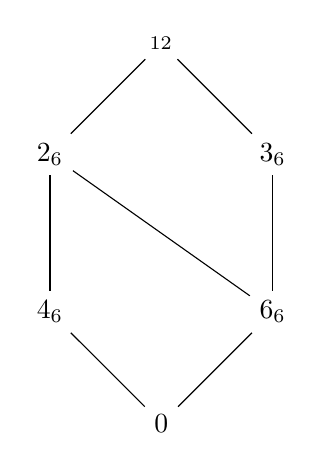
\begin{tikzpicture}
  \node (Z12) {$\integers_{12}$};
  \node (Z6) [below left of=Z12, node distance=2cm] {$2 \integers_6$};
  \node (Z4) [below right of=Z12, node distance=2cm] {$3 \integers_6$};
  \node (Z3) [below of=Z6, node distance=2cm] {$4 \integers_6$};
  \node (Z2) [below of=Z4, node distance=2cm] {$6 \integers_6$};
  \node (0) [below left of=Z2, node distance=2cm] {0};
  \path[-]  (Z12) edge node {} (Z6)
            (Z12) edge node {} (Z4)
            (Z6) edge node {} (Z2)
            (Z6) edge node {} (Z3)
            (Z4) edge node {} (Z2)
            (Z2) edge node {} (0)
            (Z3) edge node {} (0)
            ;
\end{tikzpicture}
\caption{Reticolo dei sottogruppi di $Z_{12}$}
\end{figure}


Reticolo dei sottogruppi di $Z_n$

$(\subgroupset(Z_n), \subseteq)$ % fare la fancy S

\begin{esercizio}
Creare il reticolo dei sottogruppi di $Z_16$.

\vskip 5cm
\end{esercizio}

\begin{defn}
Un gruppo $(G, \cdot)$ si dice ciclico, se $G = \pow{a}$, ossia $G = \{ a^{t} : t \in Z \}$, ossia $G$ \`e generato da un elemento $a \in G$ detto generatore.

L'ordine di $G$ \`e l'ordine di $a$, ossia il minimo intero tale per cui $a$ elevato all'ordine fa $1_G$, ossia $\inf \{ t > 0 e a^t = 1_G \}$
\end{defn}

$(Z, +)$ \`e ciclico, generato da $\pow{1}$. Anche $(Z_n, +)$ \`e generato da $\{ 1 \}$.

\begin{theorem}
Sia $(G, \cdot)$ un gruppo ciclico generato da $a \in G$, allora ci sono due casi:
\begin{enumerate}
    \item\label{itm:gruppo_ciclico_infinito} $\abs{G} = \infty$
    \item\label{itm:gruppo_ciclico_finito} $\abs{G} = n$, ossia la sua cardinalit\`a \`e finita
\end{enumerate}
Nel caso \ref{itm:gruppo_ciclico_infinito} $(G,+)$ \`e isomorfo a $(Z,+)$. Nel caso \ref{itm:gruppo_ciclico_finito}, $(G, +)$ \`e isomorfo a $(Z_n, +)$.
\end{theorem}

\begin{proof}
Dimostrazione dei due casi.

Caso \ref{itm:gruppo_ciclico_infinito}. Troviamo $f : (Z, +) \to (G, \cdot)$. $G = \pow{a}$. L'isomorfismo \`e l'unico che esiste tale per cui $f(1) = a$. Ossia $f(t) = a^{t}$.
\[
f(-t) = a^{-t} = (a^t)^{-1}
\]
\`E un morfismo per la propriet\`a delle potenze. Inoltre $f$ \`e suriettivo.

Bisogna dimostrare che \`e un isomorfismo, ossia che $f$ \`e iniettivo.
\[
f(t) = f(s) \implies f(t) = a^t = a^s = f(s) \implies a^t \cdot a^{-s} = 1_G \implies a^{t - s} = 1_G 
\]
Siamo nel caso in cui $\abs{G} = \infty$, quindi $a^t \neq 0 \forall t \neq 0$. Quindi
\[
t - s = 0 \implies t = s
\]
Caso \ref{itm:gruppo_ciclico_finito}. $\abs{G} = n, G = \{a^t : t \in Z\} = \pow{a}$

Dobbiamo trovare il morfismo $f : (Z_n, +) \to (G, \cdot)$, l'unico per cui $f(1) = a$ e $f(t) = a^t$ con $t \in Z_n$.

\`E suriettivo perch\'e $Z_n$ contiene tutte le potenze. Bisogna dimostrare che \`e iniettivo.

$f(t) = f(s)$, con $t, s \in Z_n$. Quindi $a^t = a^s$, quindi $a^{t-s} = 1_G$. Sappiamo che:
\[
a^n = 1_G
\]
Se considero $t - s = q \cdot n + r, a^{t-s} = a^{qn} \cdot a^{r} = 1_G \implies 1_G \cdot a^{r} \implies a^r = a^0$

Quindi deve essere che $(t - s) \equiv 0 \pmod{n}$.

$f(t) = f(s) \implies a^t = a^s \implies a^{t-s} = 1_G \implies a^{t-s} = a^{qn + r} = 1_G$. Ho che $0 \le r < n$. Quindi$ 1_G = a^{qn} \cdot a^r$, ma $a^{qn} = 1_G$, quindi $1_G = 1_G \cdot a^r \implies a^r = a^0$, essendo $r < n$.

Quindi essendo $r = 0, (t - s) = qn$, quindi $t - s \equiv 0 \pmod{n}$, ossia che $t - s = 0$ in $Z_n$.
\end{proof}

\begin{esercizio}
Scrivere le tavole moltiplicative dei tre gruppi $U(Z_5)$, $U(Z_8)$ e $U(Z_10)$. Calcolare la cardinalit\`a dei suddetti gruppi, e di $U(Z_12)$.

Determinare quali sono isomorfi, esplicitando l'isomorfismo.
\[
U(Z_5) = \{ 1, 2, 3, 4 \}
\]
\begin{tabular}{c|*{4}{c}}
$\cdot$ & 1 & 2 & 3 & 4 \\
\hline
1 & 1 & 2 & 3 & 4 \\
2 & 2 & 4 & 1 & 3 \\
3 & 3 & 1 & 4 & 2 \\
4 & 4 & 3 & 2 & 1
\end{tabular}
\begin{align*}
o(2) &= 4 \iff 2^4 = 16 \equiv 1 \pmod{5} \\
o(3) &= 2 \iff 3^2 = 6 \equiv 1 \pmod{5} \\
o(4) &= 2 \iff 4^2 = 16 \equiv 1 \pmod{5}
\end{align*}
\[
U(Z_5) = \pow{2} \cong Z_4
\]
\[
U(Z_8) = \{ 1, 3, 5, 7 \}
\]
\begin{tabular}{c|*{4}{c}}
$\cdot$ & 1 & 3 & 5 & 7 \\
\hline
1 & 1 & 3 & 5 & 7 \\
3 & 3 & 1 & 7 & 5 \\
5 & 5 & 7 & 1 & 3 \\
7 & 7 & 5 & 3 & 1
\end{tabular}
\[
U(Z_10) = \{ 1, 3, 7, 9 \}
\]
\begin{tabular}{c|*{4}{c}}
$\cdot$ & 1 & 3 & 7 & 9 \\
\hline
1 & 1 & 3 & 7 & 9 \\
3 & 3 & 9 & 1 & 7 \\
7 & 7 & 1 & 9 & 3 \\
9 & 9 & 7 & 3 & 1
\end{tabular}
\[
U(Z_12) = \{ 1, 5, 7, 11 \}
\]
\[
o(3) = 4 \iff 3^4 = 81 \equiv 1 \pmod{10}
\]
\[
U(Z_10) = \pow{3} \cong Z_4
\]
C'\`e un isomorfismo fra $U(Z_5)$ e $U(Z_10)$. Il generatore deve andare nel generatore, il quadrato del generatore nel quadrato del generatore, etc.

\begin{figure}
\centering
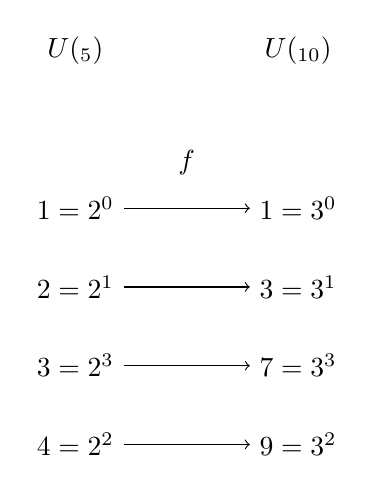
\begin{tikzpicture}
  \node (UZ5) {$U(\integers_5)$};
  \node (f) [below right of=UZ5, node distance=2cm] {$f$};
  \node (UZ10) [above right of=f, node distance=2cm] {$U(\integers_{10})$};
  \node (5_0) [below of=UZ5, node distance=2cm] {$1 = 2^0$};
  \node (5_1) [below of=5_0, node distance=1cm] {$2 = 2^1$};
  \node (5_2) [below of=5_1, node distance=1cm] {$3 = 2^3$};
  \node (5_3) [below of=5_2, node distance=1cm] {$4 = 2^2$};
  \node (10_0) [below of=UZ10, node distance=2cm] {$1 = 3^0$};
  \node (10_1) [below of=10_0, node distance=1cm] {$3 = 3^1$};
  \node (10_2) [below of=10_1, node distance=1cm] {$7 = 3^3$};
  \node (10_3) [below of=10_2, node distance=1cm] {$9 = 3^2$};
  \path[->]  (5_0) edge node {} (10_0)
            (5_1) edge node {} (10_1)
            (5_2) edge node {} (10_2)
            (5_3) edge node {} (10_3)
            ;
\end{tikzpicture}
\caption{L'isomorfismo tra $U(\integers_5)$ e $U(\integers_{10})$}
\end{figure}

\begin{tabular}{c|*{4}{c}}
$\cdot$ & 1 & 5 & 7 & 11 \\
\hline
1 & 1 & 5 & 7 & 11 \\
5 & 5 & 1 & 11 & 7 \\
7 & 7 & 11 & 1 & 5 \\
11 & 11 & 7 & 5 & 1
\end{tabular}
\begin{align*}
o(5) &= 2 \iff 5^2 = 25 \equiv 1 \pmod{12} \\
o(7) &= 2 \iff 7^2 = 49 \equiv 1 \pmod{12} \\
o(11) &= 2 \iff 11^2 = 121 \equiv 1 \pmod{12}
\end{align*}
Quindi $U(Z_12)$ non \`e un gruppo ciclico. Vediamo se \`e isomorfo a $Z_8$.

$Z_8$ deve avere tre elementi di ordine 2.
\begin{align*}
o(3) &= 2 \iff 3^2 = 9 \equiv 1 \pmod{8} \\
o(5) &= 2 \iff 5^2 = 25 \equiv 1 \pmod{8} \\
o(7) &= 2 \iff 7^2 = 49 \equiv 1 \pmod{8}
\end{align*}
Quindi $Z_8$ e $Z_12$ sono isomorfi.
\end{esercizio}

\begin{esercizio}
Risolvere la congruenza:
\[
511 x \equiv 111 \pmod{842}
\]
Scrivere le soluzioni modulo 842.
\end{esercizio}

\begin{esercizio}
Calcolare $2^{2341} \pmod{37}$.
\end{esercizio}



























